\pdfoutput=1

\documentclass{l4proj}
\usepackage{url}
\usepackage{subcaption}
\usepackage{float}
% compacting the list items
\usepackage{enumitem}
\usepackage{multirow}
\usepackage{booktabs}
\usepackage{tabularx} % in the preamble
\usepackage{adjustbox}
\usepackage{multicol}
\usepackage{pdfpages}


% code
\usepackage{listings}
\usepackage{color}
\usepackage{textcomp}
\definecolor{listinggray}{gray}{0.9}
\definecolor{lbcolor}{rgb}{0.9,0.9,0.9}
\lstset{
	language        = php,
	emph            =[1]{php},
	emph            =[2]{if,and,or,else},
	backgroundcolor=\color{lbcolor},
	tabsize=4,
	rulecolor=,
	language=matlab,
	basicstyle=\scriptsize,
	upquote=true,
	aboveskip={1.5\baselineskip},
	columns=fixed,
	showstringspaces=false,
	extendedchars=true,
	breaklines=true,
	prebreak = \raisebox{0ex}[0ex][0ex]{\ensuremath{\hookleftarrow}},
	frame=single,
	showtabs=false,
	showspaces=false,
	showstringspaces=false,
	identifierstyle=\ttfamily,
	keywordstyle=\color[rgb]{0,0,1},
	commentstyle=\color[rgb]{0.133,0.545,0.133},
	stringstyle=\color[rgb]{0.627,0.126,0.941},
}

%
% put any packages here
%

\begin{document}
\title{Urban Data Timeline}
\author{Yordan Yordanov}
\date{March 28, 2016}
\maketitle

\begin{abstract}
We show how to produce a level 4 project report using latex and pdflatex using the 
style file l4proj.cls
\end{abstract}

\educationalconsent
%
%NOTE: if you include the educationalconsent (above) and your project is graded an A then
%      it may be entered in the CS Hall of Fame
%
\tableofcontents
%==============================================================================

\chapter{Introduction}
\pagenumbering{arabic}

\section{Motivations}
\paragraph{}
Smart cities bring a lot of advantages. They can opt for better urban planning and development by making more efficient use of the infrastructure to improve productivity and services but also to reduce the waste of fuel and energy. Furthermore their intelligence can change and enhance the way authorities respond to changing circumstances. On the other hand, achieving all these goals is a challenging process. Huge amounts of information, created by social feeds, environmental sensors, traffic, news and many more, have to be gathered, stored and analysed. This project aims to combine and visualise all these data strands so that some can look at the cities from a different angle and possibly extract new tendencies and patterns, not possible to discover by following only a single source. This will help us identify problems or challenges that we had not been aware of and provide effective solutions that we all as citizens can only benefit from.

\section{Aims}
\label{sec:aims}
\paragraph{}
This project aims to build a tool for the fusion and visualisation of timely data collected from the Urban Big Data Centre for their Integrated Multimedia City Data project. Past data from various urban data streams, such as social media posts, news, blogs, traffic information, environmental sensors and many more has been provided. The tool should be able to query all this data and come up with a timeline representation of observations that might be of interest to the user. This application is initially build to be used by the general public but may as all be valuable to local researchers who follow or compare people’s opinions, businessmen who want to know how their business is developing, media that want to report what are the public impressions about an important event and even politicians while running their campaigns.   

\section{Background}
\paragraph{}
Smart cities today represent a perception to integrate both information and communication technologies in an acceptable and maintainable fashion to manage their infrastructure and facilities. The optimal goal is to enhance the quality of life and satisfy the residents’ needs. ICT gives to the people, who maintain these cities, the great opportunity to directly follow what is happening and take actions accordingly. This can be done only by processing the huge amounts of information, collected from sensors, in real time and providing knowledge and information: the keys for discovering inefficiencies. 
\paragraph{}
However, the biggest asset of a smart city is not the number of cameras or sensors but the people that occupy it. A third of the internet users\cite{ofcomreport1} represent their smart-phone as the most important device for going online. A third of the population owns a smart device and use it every day to bank, shop and access social media. Social media streams, such as Twitter, have a reputation to be extremely useful source of information. Anybody can understand what is happening all around the world in real time. With that comes various opportunities for developers to implement systems that automatically detect and track events as they happen. Smart cities can benefit from that as what better way to improve efficiency than for example identifying and reporting road accidents to the emergency services in real time.
\paragraph{}
Aiming to help with analysing these massive amounts of data, the Urban Big Data Centre was established by the UK Economic and Social Research Council to address social, economic and environmental challenges facing cities. Their researchers are undertaking innovative projects, covering topics from big data management to linking and analysing the multi-structural urban data.  Such project is the Integrated Multimedia City Data. 



\subsection{Integrated Multimedia City Data}

\paragraph{}
Integrated Multimedia City Data\cite{imcd} (iMCD) is one of the Urban Big Data Centre’s inaugural projects, funded by the Economic and Social Research Council. It is designed to provide the UBDC with innovative primary data sources. The project consists of four strands: representative household survey, tracking of real-time urban sensors, internet based visual and textual media collection.  
\paragraph{}
The core research strand is the representative household survey that aims to gather data about people’s attitude and behaviour when it comes to information and communication technologies, travelling and learning. Some of the participants are given GPS and life logging sensors that record their activities and travel. Meanwhile the visual and textual data, referring to Glasgow and surrounding areas, is to be collected from the internet. 
\paragraph{}
All of these strands, together, are able to show how Glasgow performs as a smart city.  The Terrier IR team provides various data web services so that all these sources can be browsed and queried.

\subsection{Terrier IR}
\paragraph{}
Terrier IR\footnote{\url{http://terrierteam.dcs.gla.ac.uk/}} team consists of researchers, working on large-scale textual information retrieval. They are part of the Computer Science Department at the University of Glasgow. The Terrier IR Platform\footnote{\url{http://terrier.org/}} is where they concentrate their research. It is an open source search engine that is highly effective and ready to be used on large-scale collections of documents. 

\subsection{RESTful Web Services}
\paragraph{}
Web technologies are not meant to only deliver HTML pages between HTTP clients but also, with their technical fundamentals of URIs, HTML and HTTP, to provide a widely deployed information delivery and service platform. REST, on the other hand, is a set of constraints that guide the design of such systems. The general claim of RESTful systems, implementing these constraints, are that they are highly scalable and that the interlinking of self-describing representation formats allows such a system to grow organically and in a decentralized way\cite{restful}. As the time of writing, REST is one of the most important technologies that is used in many Web and Mobile applications.

\subsection{Web Application}
\paragraph{}
Web application runs in a web browser and follows the client-server model(\ref{fig:clientserver}). It is based on splitting the tasks or workloads between a provider, called server, and a requester, called client. Web applications can run on every platform as far as there is a web browser. This is a great relief for the developers as there are far less constraints on the implementation. Web applications usually are built from a combination of  server-side and client-side scripts. The server-side scripts take care of storing, processing and retrieving information while the client-side is responsible for presenting it. Furthermore, the separation of concerns allows for updates to be made independently.    

\begin{figure}[H]
	\centering
	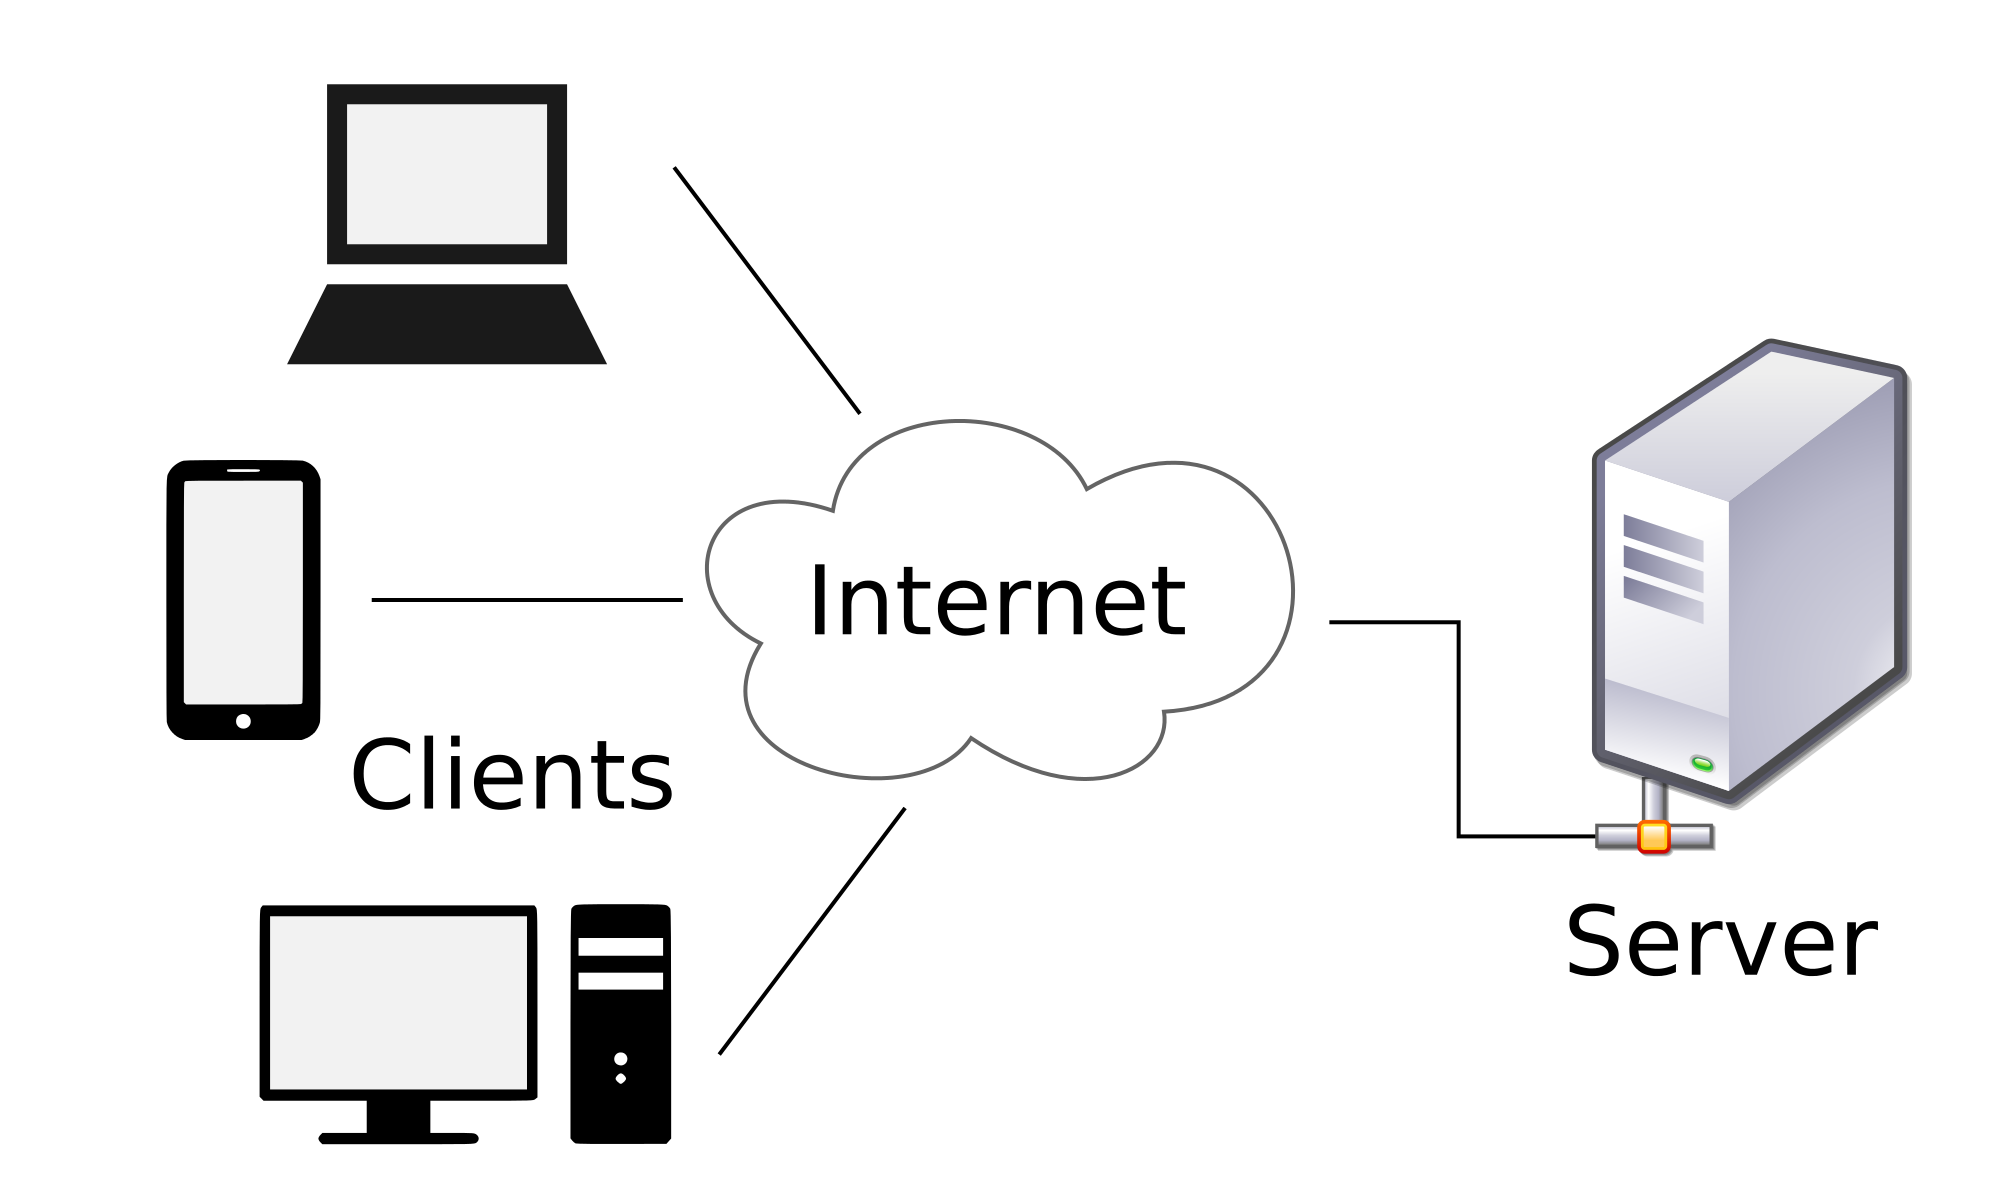
\includegraphics[width=.5\textwidth]{images/clientserver}
	\caption{Client-Server Model}
	\label{fig:clientserver}
\end{figure} 

\section{Outline}
The rest of the report is structured as follows:
\begin{itemize}
	\item \textbf{Chapter 2} provides an overview of related work with examples of similar applications.
	
	\item \textbf{Chapter 3} discusses the project planning by separating it into design approach and requirements engineering.
	\item \textbf{Chapter 4} explains the design by showing the initial paper prototypes and architectural diagrams. It also provides a comparison between the possible technologies, that were available and suitable for such a project.
	\item \textbf{Chapter 5} goes through the actual implementation of each component and describes the challenges faced. 
	\item \textbf{Chapter 6} describes the two phases of the evaluation process and explains the testing strategy for the components.
	\item \textbf{Chapter 7} concludes the report and discusses the implication of the evaluations in terms of future directions
\end{itemize}


\chapter{Related Work}
\paragraph{}
There are applications that have been developed to use a timeline for presenting some kind of data. This chapter is reveals a short description of related products, along with key differences and correlations in comparison with the main ideas behind this project.  

\subsubsection{Google Maps Timeline} 
\paragraph{}
Google stores a history of where anybody that uses its location services goes. All this data is collected by your device sensors and the navigation you use. Then it is visualized with the Google Maps Timeline \cite{GoogleMapsTimeline} feature. This application is advertised to be an easy way to view and remember places somebody has been on a given day at a given time. Without any input, the timeline shows predictions of when you have arrived or left a place. One of the key features is highlighting when you have visited the most places and how you had travelled. The application does not offer sharing as Google wants your information to remain private. As far as human interaction goes, you are allowed to correct, confirm or delete a place where Google thinks you had been but even after deleting,  it can still be seen that you had passed by that area. In 2009, the company released a similar feature called Google Latitude that offered sharing of location history but the project was closed down \cite{GMTimeFeature}.

\paragraph{}
This product has the same initial goal to visualize timely data originating from different streams like navigation history, pictures, travel and walking routes. Some of the key features are using a vertical timeline to display the events, allowing searching based on a specific day, month, year and having a way to show (via bar chart) how active you have been every day in the past few weeks. 

\subsubsection{Social Media Timeline}
\paragraph{}
All social media websites in the likes of Twitter and Facebook use some sort of a timeline to visualize their user's personal information. However they differ on the way they organize their posts. Facebook describes a timeline to be a place on your profile where you can see your own posts, your friends' activities and stories you're tagged in, sorted by the date and time they were posted. On the other hand, Twitter displays a stream of tweets from accounts that you have chosen to follow. Making use of machine learning algorithms, posts that you are likely to care about more are displayed first.
\paragraph{}
Despite the fact that social media applications have as a main goal the delivery of a secure and reliable tool for communication, they also provide their users with the ability to visualize their personal data streams like photos, events, group activities and accomplishments. Both Facebook and Twitter use a vertical timeline and allow for searching based on keywords. One of the key features is infinite scrolling that make the illusion of one endless stream of events by making use of the million users, posting every day. 

\subsubsection{Tech City Map}
\paragraph{}
Tech City Map pulls streams of social media posts for all the businesses in the East London area and tries to analyse their influence. The idea lies on using a map to display all the corporations in the area and linking them together by using different coloured lines for any tweet from one business to the other. The tool allows searching for a specific company as some points represents more then one corporation and manually searching though the map can be difficult. From 2010 to 2012\footnote{\url{http://flowingcity.com/visualization/tech-city-map/}} the number of businesses in East London had risen from 200 to 600. This growth was welcomed even by the Prime Minister at that time, David Cameron, proving that such tools are even followed by politicians. 

\subsubsection{Summary}
\label{subsubsec:conclusion}
\paragraph{}
Some of the previously described applications are proven to be successful by millions of users all around the world. However, they focus only on their user and do not really visualise and offer a big variety of data sources. On the other hand, Urban Data Timeline targets the smart city by increasing the user's understating about it. Furthermore, with the help of the Urban Big Data Centre, it has plenty data streams to offer: querying a tweet collection based on a hash-tag or specific tweet terms, examining the events, detected by automated systems, related to specific terms, obtaining information about busy venues in an area of a city, finding train stations within a radius of a specific location, searching for delayed trains and accessing past weather data records. Also, all these big companies like Google, Facebook and Twitter provide their own APIs. This brings a great opportunity for this innovative project to become a centralised system where, for example, busy venues can be listed with the tweets from their own Twitter or Facebook accounts and events can be reviewed in depth with the help of news and youtube videos. On the other hand, the next chapter describes how the project was planned and lists the identified use cases, requirements and challenges along with a high level diagram of the system. 


\chapter{Project Planning}

\section{Software design approach}
\paragraph{}
When a new product is developed, it is not clear how it will end up and if it will fulfil the user's requirements. The developers can see the first steps but there are plenty of problems or challenges that can not be predicted from the beginning (Figure \ref{projectInitial}). That is true for any project, no matter how much planning is put in. However there is a possibility that everything is done the right way but there is a high probability to drift away from the initial target (Figure \ref{projectStart}). There are several methodologies that can be followed when developing a software but the two most common are Waterfall and Agile. 

\subsection{Waterfall model}
\paragraph{}
The Waterfall model is an example of a plan-driven process - in principle you must plan and schedule all of the process activities before starting work on them \cite{sene}. Here iterations can be costly and involve significant rework. Therefore, after a small number of iterations, it is normal to freeze parts of the development, such as the specification, and continue with the later development stages. Problems are left for later resolution, programmed around or completely ignored. These implementation tricks may also lead to design problems and badly structured systems.

\subsection{Agile model}
\paragraph{}
This project, on the other hand, follows the Agile methodology (Figure \ref{projectAgile}) for software development. It is an interactive
approach that splits the work into a number of iterations (sprints). This allow the project supervisors to inspect the work of the developer and monitor how well the software development is progressing \cite{sene}. Each of these sprints last one
week. It starts with a meeting and demonstration of the work done in the previous sprint. As an
outcome of these meetings feedback from the supervisors is received, based on the
extent to which their requirements are met. Moreover, these meetings allow discussions of the issues
that are experienced and compare the available workarounds. At the end of a meeting, it is agreed
upon exactly what work will be done during the next sprint. Following this scenario, at least one new
feature is introduced after each sprint and changes to previous features are performed as early as possible. By the end of this project, 23 iterations are to be performed.

\begin{figure}[H]
\begin{subfigure}{.3\textwidth}
	\centering
	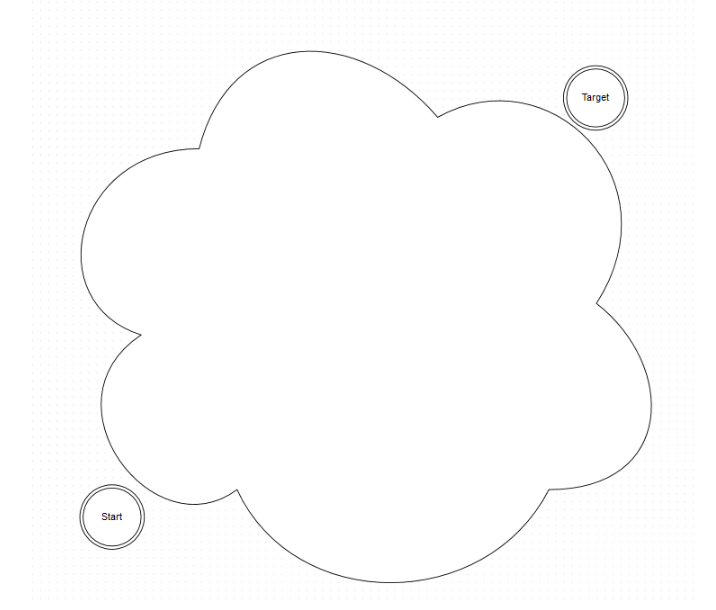
\includegraphics[width=\textwidth]{images/projectInitial}
	\caption{Start of a project.}
	\label{projectInitial}
\end{subfigure}
\begin{subfigure}{.3\textwidth}
	\centering
	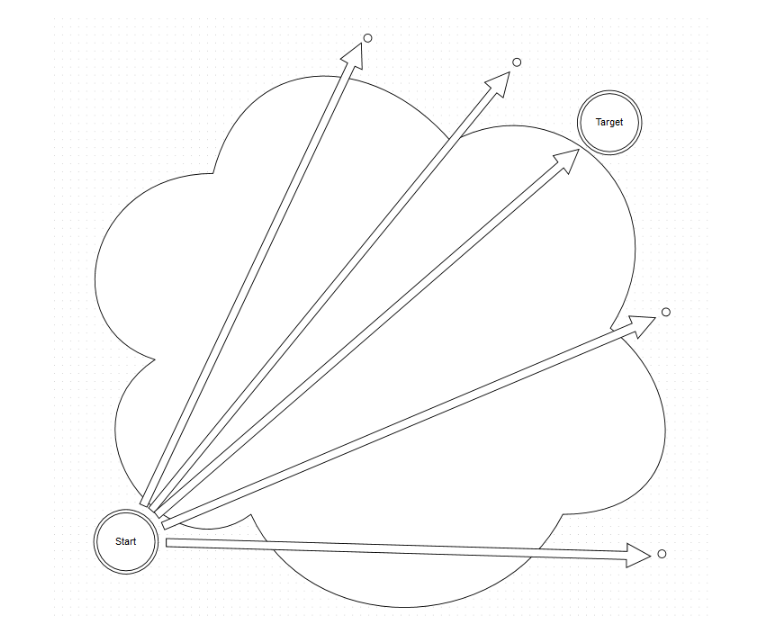
\includegraphics[width=\textwidth]{images/projectStart}
	\caption{Waterfall methodology.}
	\label{projectStart}
\end{subfigure}
\begin{subfigure}{.3\textwidth}
	\centering
	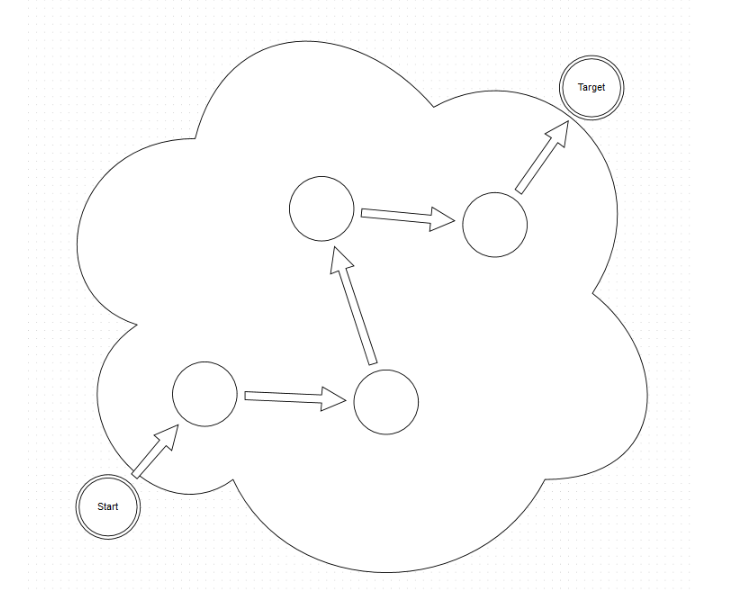
\includegraphics[width=\textwidth]{images/projectAgile}
	\caption{Agile methodology.}
	\label{projectAgile}
\end{subfigure}
\caption{Software development methodologies}
\end{figure}



\section{Requirements Engineering}
\paragraph{}
The requirements for a system describes the functionality of the services it provides and the constraints of its operation. The process of gathering, analysing and documenting these services and constraints is called requirements engineering.
\paragraph{}
At the beginning of the project, a few weeks were taken to envision the high-level requirements and to understand the scope of the required system. For the initial requirements use cases and user stories were extracted to help with exploring how users will work with the system. 

\subsection{Use cases} 
\label{sec:usecases}
\paragraph{}
Use case is a way to describe how a real user interacts with the system. They should not be perfect and can only show the action and not go into much detail, in order to stay close to the agile methodology. The developer will implement the system but will have to work close with the supervisors so that the end product will meet their needs. 

The following use cases were identified in the beginning of this project: 


\begin{itemize}%[noitemsep]
	\item see how tweets about a specific hash-tag are distributed over a period of time
	\item see popular hash-tags that are twitted together with a specific hash-tag
	\item get information about a certain area of the city and find out if the venues(restaurants, train stations, cinemas) there get high attendance
	\item browse tweets based on time and hash-tag
	\item use the system on a mobile device
	\item check out what the clients post about a venue, they had visited
	\item check how many people attend specific venues in a given area
	\item compare people's opinions about an event
	\item see if a political party is likely to win the elections
\end{itemize}


\subsection{Functional requirements} 
\label{sec:functional-requirements}
\paragraph{}
Functional requirements represent services the system should provide, how it should react to particular inputs and how the system should behave in some situations. More specific requirements can describe the system functions, its inputs and output or exceptions in detail \cite{sene}. 
\paragraph{}
Adding new requirements may change the project direction. Projects usually have fixed duration so sometimes it may not be possible to include all the features. Therefore all use cases that are identified in this chapter must be prioritised. 

\begin{figure}[H]
	\centering
	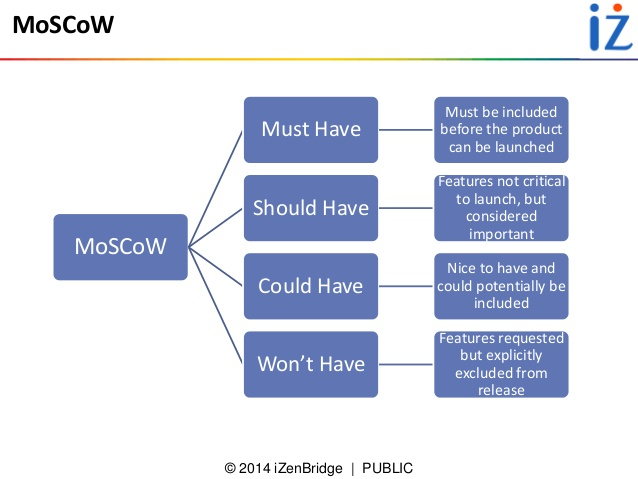
\includegraphics[width=.5\textwidth]{images/MoSCoW}
	\caption{MoSCoW rules prioritisation scheme for requirements}
	\label{MoSCoW}
\end{figure} 
\paragraph{}
Figure \ref{MoSCoW} shows the MoSCoW rules that are typically used as a guideline for prioritising requirements. All the use cases should be sorted, using these rules. The ones that are "Must Have" and "Should Have" should be feasible in the duration of the project. Table \ref{tab:funcReq} represents the extracted requirements after their prioritisation. It has now been modified according to the final list of requirements.

%\textbf{\textit{Functional Requirements}}.
%\begin{itemize}
%	\item \textit{User Interface}
%	\begin{itemize}
%		\item Must be able to display a fusion of different kinds of timely data (tweets, weather, traffic, train delays etc.).
%		\item Must be able to show specific as well as general information based on the request.
%		\item Must display events in a timeline.
%		\item Must display the time of events.
%		\item Must be able to take date input.
%		\item Must be able to receive hash-tag input.
%		\item Must be able to take location based input.
%		\item Must be able to show venues in specific area. (using a Map)
%		\item Should dynamically add data to the layout. (using AJAX)
%		\item Should be able to visualise statistic data on a graph.
%		\item Could show a summary of the made request.
%		\item Could show the link of an event with other events.
%	\end{itemize}
%	
%	\item \textit{Server}
%	\begin{itemize}
%		\item Must be able to fetch data from provided services.
%		\item Must be able to fetch data from external sources. (Twitter)
%		\item Should provide additional RESTful APIs. (TODO: explain what is REST)
%		\item Should support caching.
%		\item Could store pre-render events. 
%		
%	\end{itemize}
%\end{itemize}   

\begin{table}[ht]
	\centering
	\begin{adjustbox}{width=1\textwidth}
		\begin{tabular}{|c|@{}c@{}|}\hline
			\multicolumn{2}{|l|}{\textbf{Functional Requirements}} \\\hline
			\textbf{MoSCoW} & \textbf{User Interface} \\ \hline
			Must
			&
			\begin{tabularx}{\textwidth}{l}
				be able to display a fusion of different kinds of timely data (tweets, weather, traffic, train delays etc.). \\\hline
				be able to show specific as well as general information based on the request. \\\hline
				display events in a timeline. \\\hline
				display the time of events. \\\hline
				be able to take date input. \\\hline
				be able to receive word based input. \\\hline
				be able to take location based input. \\\hline
				be able to show venues in specific area. (using a Map) \\\hline
				be able to show two events, side by side, so that they can be compared. \\
			\end{tabularx}
			\tabularnewline\hline
			Should
			&
			\begin{tabularx}{\textwidth}{l}
				dynamically add data to the layout. (using AJAX) \\\hline
				be able to visualise statistic data on a graph. \\
			\end{tabularx}
			\tabularnewline\hline
			Could
			&
			\begin{tabularx}{\textwidth}{l}
				show a summary of the made request.	\\\hline
				show the link of an event with other events.\\
			\end{tabularx}
			\tabularnewline\hline
			
			& \textbf{Server} \\ \hline
			Must
			&
			\begin{tabularx}{\textwidth}{l}
				be able to fetch data from provided services. \\\hline
				be able to fetch data from external sources. (Twitter) \\
			\end{tabularx}
			\tabularnewline\hline
			Should
			&
			\begin{tabularx}{\textwidth}{l}
				provide additional RESTful APIs. (TODO: explain what is REST) \\\hline
				support caching. \\
			\end{tabularx}
			\tabularnewline\hline
			Could
			&
			\begin{tabularx}{\textwidth}{l}
				store pre-render events. \\
			\end{tabularx}
			\tabularnewline\hline
			
		\end{tabular}
	\end{adjustbox}
	\caption{Functional Requirements}
	\label{tab:funcReq}
\end{table}


\subsection{Non-Functional requirements}
\paragraph{}
Non-functional requirements represent constraints on the services or functions offered by the system. They often apply to the application as a whole, rather than individual components \cite{sene}. Table \ref{tab:nonFuncReq} represents the extracted non-functional requirements for this project. 

%	\textbf{\textit{Non-Functional Requirements}}.
%	\begin{itemize}
%		\item Must be universal to support all kinds of users(citizen, scientist, researchers, local authorities)
%		\item Must be extensible so that different things can be rendered on the views.
%		\item Must be able to quickly process the data from the services.
%		\item Should be accessible from and compatible with desktops, laptops, tablets and smartphone devices.
%		\item Should be testable.
%		\item Should be scalable so that new services can be added.
%		\item Could be compatible with tools that can measure code quality. (Sonar)
%	\end{itemize}

\begin{table}[ht]
	\centering
	\begin{adjustbox}{width=1\textwidth}
		\begin{tabular}{|c|@{}c@{}|}\hline
			\multicolumn{2}{|l|}{\textbf{Non-Functional requirements}} \\\hline
			\textbf{MoSCoW} & \textbf{Requirement} \\ \hline
			Must
			&
			\begin{tabularx}{\textwidth}{l}
				be universal to support all kinds of users(citizen, scientist, researchers, local authorities). \\\hline
				be extensible so that different things can be rendered on the views. \\\hline
				be able to quickly process the data from the services. \\
			\end{tabularx}
			\tabularnewline\hline
			Should
			&
			\begin{tabularx}{\textwidth}{l}
				be accessible from and compatible with desktops, laptops, tablets and smartphone devices. \\\hline
				be testable. \\\hline
				be scalable so that new services can be added. \\
			\end{tabularx}
			\tabularnewline\hline
			Could
			&
			\begin{tabularx}{\textwidth}{l}
				be compatible with tools that can measure code quality. (Sonar) \\
			\end{tabularx}
			\tabularnewline\hline
		\end{tabular}
	\end{adjustbox}
	\caption{Non-Functional Requirements}
	\label{tab:nonFuncReq}
\end{table}
	
\subsection{High Level System Diagram}
\label{sec:highLevelDiagram}
\paragraph{}
The outlined requirements and use cases start to reveal what the system architecture is going to be. In order to achieve the goals, the application has to consist of three main components (Figure: \ref{highLevelDiagram}): client to	handle the	interaction with the user, middleware to handle the application logic, and a database, in our case external services, to store the data. This architectural model is also called Three Tier Architecture. Tiers enable separation of concerns and encapsulate complexity as they can be broken down into layers and sub-tiers. Furthermore, they can be distributed across a number of machines to provide flexibility and can be replicated across a number of machines to provide the really important scalability factor\cite{threetier}.   	

\begin{figure}[H]
		\centering
		\includegraphics[width=.7\linewidth]{images/HighLevelDiagram}
		\caption{High level architecture diagram based on requirements and use cases.}
		\label{highLevelDiagram}
\end{figure}

\subsection{Challenges}
\paragraph{}
After summarising the requirements(Section: \ref{sec:functional-requirements}) and the high level diagram(Section: \ref{sec:highLevelDiagram}), some challenges can be identified. The biggest on is building a system that can be used by people without any experience in computing like citizens and satisfies the needs of researchers. Furthermore, the system should be valuable and usable on mobile devices. Taking into account how many services are to be used, the user interface must be designed carefully and efficiently. Additionally, the services are not implemented specifically for these application so a lot of unrelated data has to be filtered out. Moreover, there are multiple services and all the data, received from them, has to be sorted quickly.   

\subsection{User Stories}
\label{sec:userstories}
\paragraph{}
User stories are one of the primary development artefacts for Agile project teams. A user story is a high-level definition of a requirement, containing just enough information so that the developer can get a feel of what the user wants to achieve when using the system and performing a task. It represents a functionality that will be of a value to the user. A suggested template for a user story is: 

\begin{center}
	As a \textbf{\textit{ROLE}}, I want to \textbf{\textit{ACTION}}, so that \textbf{\textit{GOAL}}. \cite{sets}
\end{center}
\paragraph{}
The role represents the user that interacts with the system. The action shows how the user wants to use the system and the goal- what the user is trying to accomplish. All user stories are written in a way that they are understandable by both developer and customer. Ideally the customer should write the user stories while discussing them with the developer \cite{sets}. The following list represents the user stories, captured for this project based on the identified target users:    

\begin{itemize}%[noitemsep]
	\item \textbf{\textit{Researcher}}.
	\begin{itemize}
		\item As a Researcher, I would like to see how the tweets for certain query are distributed though out a period of time, so that I can see the pick of the number of tweets.
		\item As a Researcher, I would like to know other popular twitter hash-tags for a certain day, so that I can see what was interesting for the Twitter users for that day.
		\item As a Researcher, I would like to know if specific area of the city was busy on a specific date, so that I can see if specific event or weather conditions had affected that area.
		\item As a Researcher, I would like to see a timeline representation of the tweets for a specific query, so that I can follow and see if the user’s opinions change.
		\item As a Researcher, I would like to use the app on a mobile device, so that when I travel, I can continue working on my research.
		\item As a Researcher, I would like to know what were the weather conditions on a specific date and see traffic information, so that I can use the data as an experiment and measure the likelihood of using the public transport when the weather conditions are bad. 
	\end{itemize}
	
	\item \textbf{\textit{Business owner}}.
	\begin{itemize}
		\item As a Restaurant owner, I would like to see if posting a tweet on my timeline affects the number of people that attend my restaurant.
		\item As a Restaurant owner, I would like to see other venues in my area, so that I can check their attendance and try to improve mine.
		\item As a TV channel owner, I would like to compare how many people are talking about my channel at specific time, compared to other channels so that I can change my TV guide and increase my audience.
	\end{itemize}
	
	\item \textbf{\textit{Politician}}.
	\begin{itemize}
		\item As a politician, I would like to compare how popular is my party in the social media in comparison to other parties, so that I can change my campaign and increase my chances of winning.
	\end{itemize}
	
	\item \textbf{\textit{Citizen}}.
	\begin{itemize}
		\item As a citizen, I would like to compare two different public opinions about a specific event, so that I can make a decision of my own. 
	\end{itemize}
\end{itemize}

\section{Summary}
Finally, this chapter defines what design approach was used for the duration of the project. Furthermore, it lists the identified use cases and requirements, along with their representation as user stories. On the other hand, the next chapter goes though the design process and describes how the application was going to meet the requirements and outlines what was the chosen combination of technologies to solve the challenges, identified in this chapter.




\chapter{Design}

%\chapter{Solution}
\section{Paper prototypes}
\label{sec:paper-prototypes}
\paragraph{}
As shown in Figure \ref{uiPrototyping}, designing an interface prototype is an iterative process that consists of four steps. The fist step is determining the needs of the users. This is already discussed in the previous chapter. The second step is building the actual prototype. It is good to start from sketches. Once a sketch (Figure: \ref{initialPaperPrototype}) was completed, a wireframe (Figure: \ref{initialWireframe}) was prepared to be evaluated during the next meeting so that changes can be made before the start of the implementation. 

\begin{figure}[H]
	\begin{subfigure}{.33\textwidth}
		\centering
		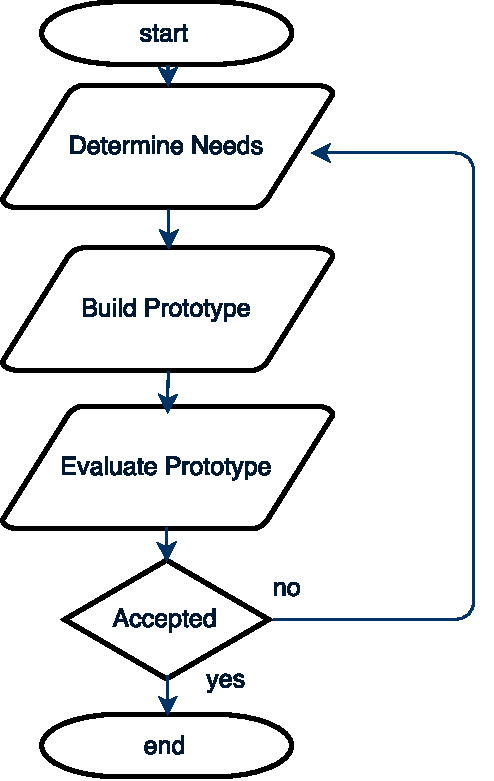
\includegraphics[width=\textwidth]{images/uiPrototyping}
		\caption{Prototyping process}
		\label{uiPrototyping}
	\end{subfigure}
	\begin{subfigure}{.33\textwidth}
		\centering
		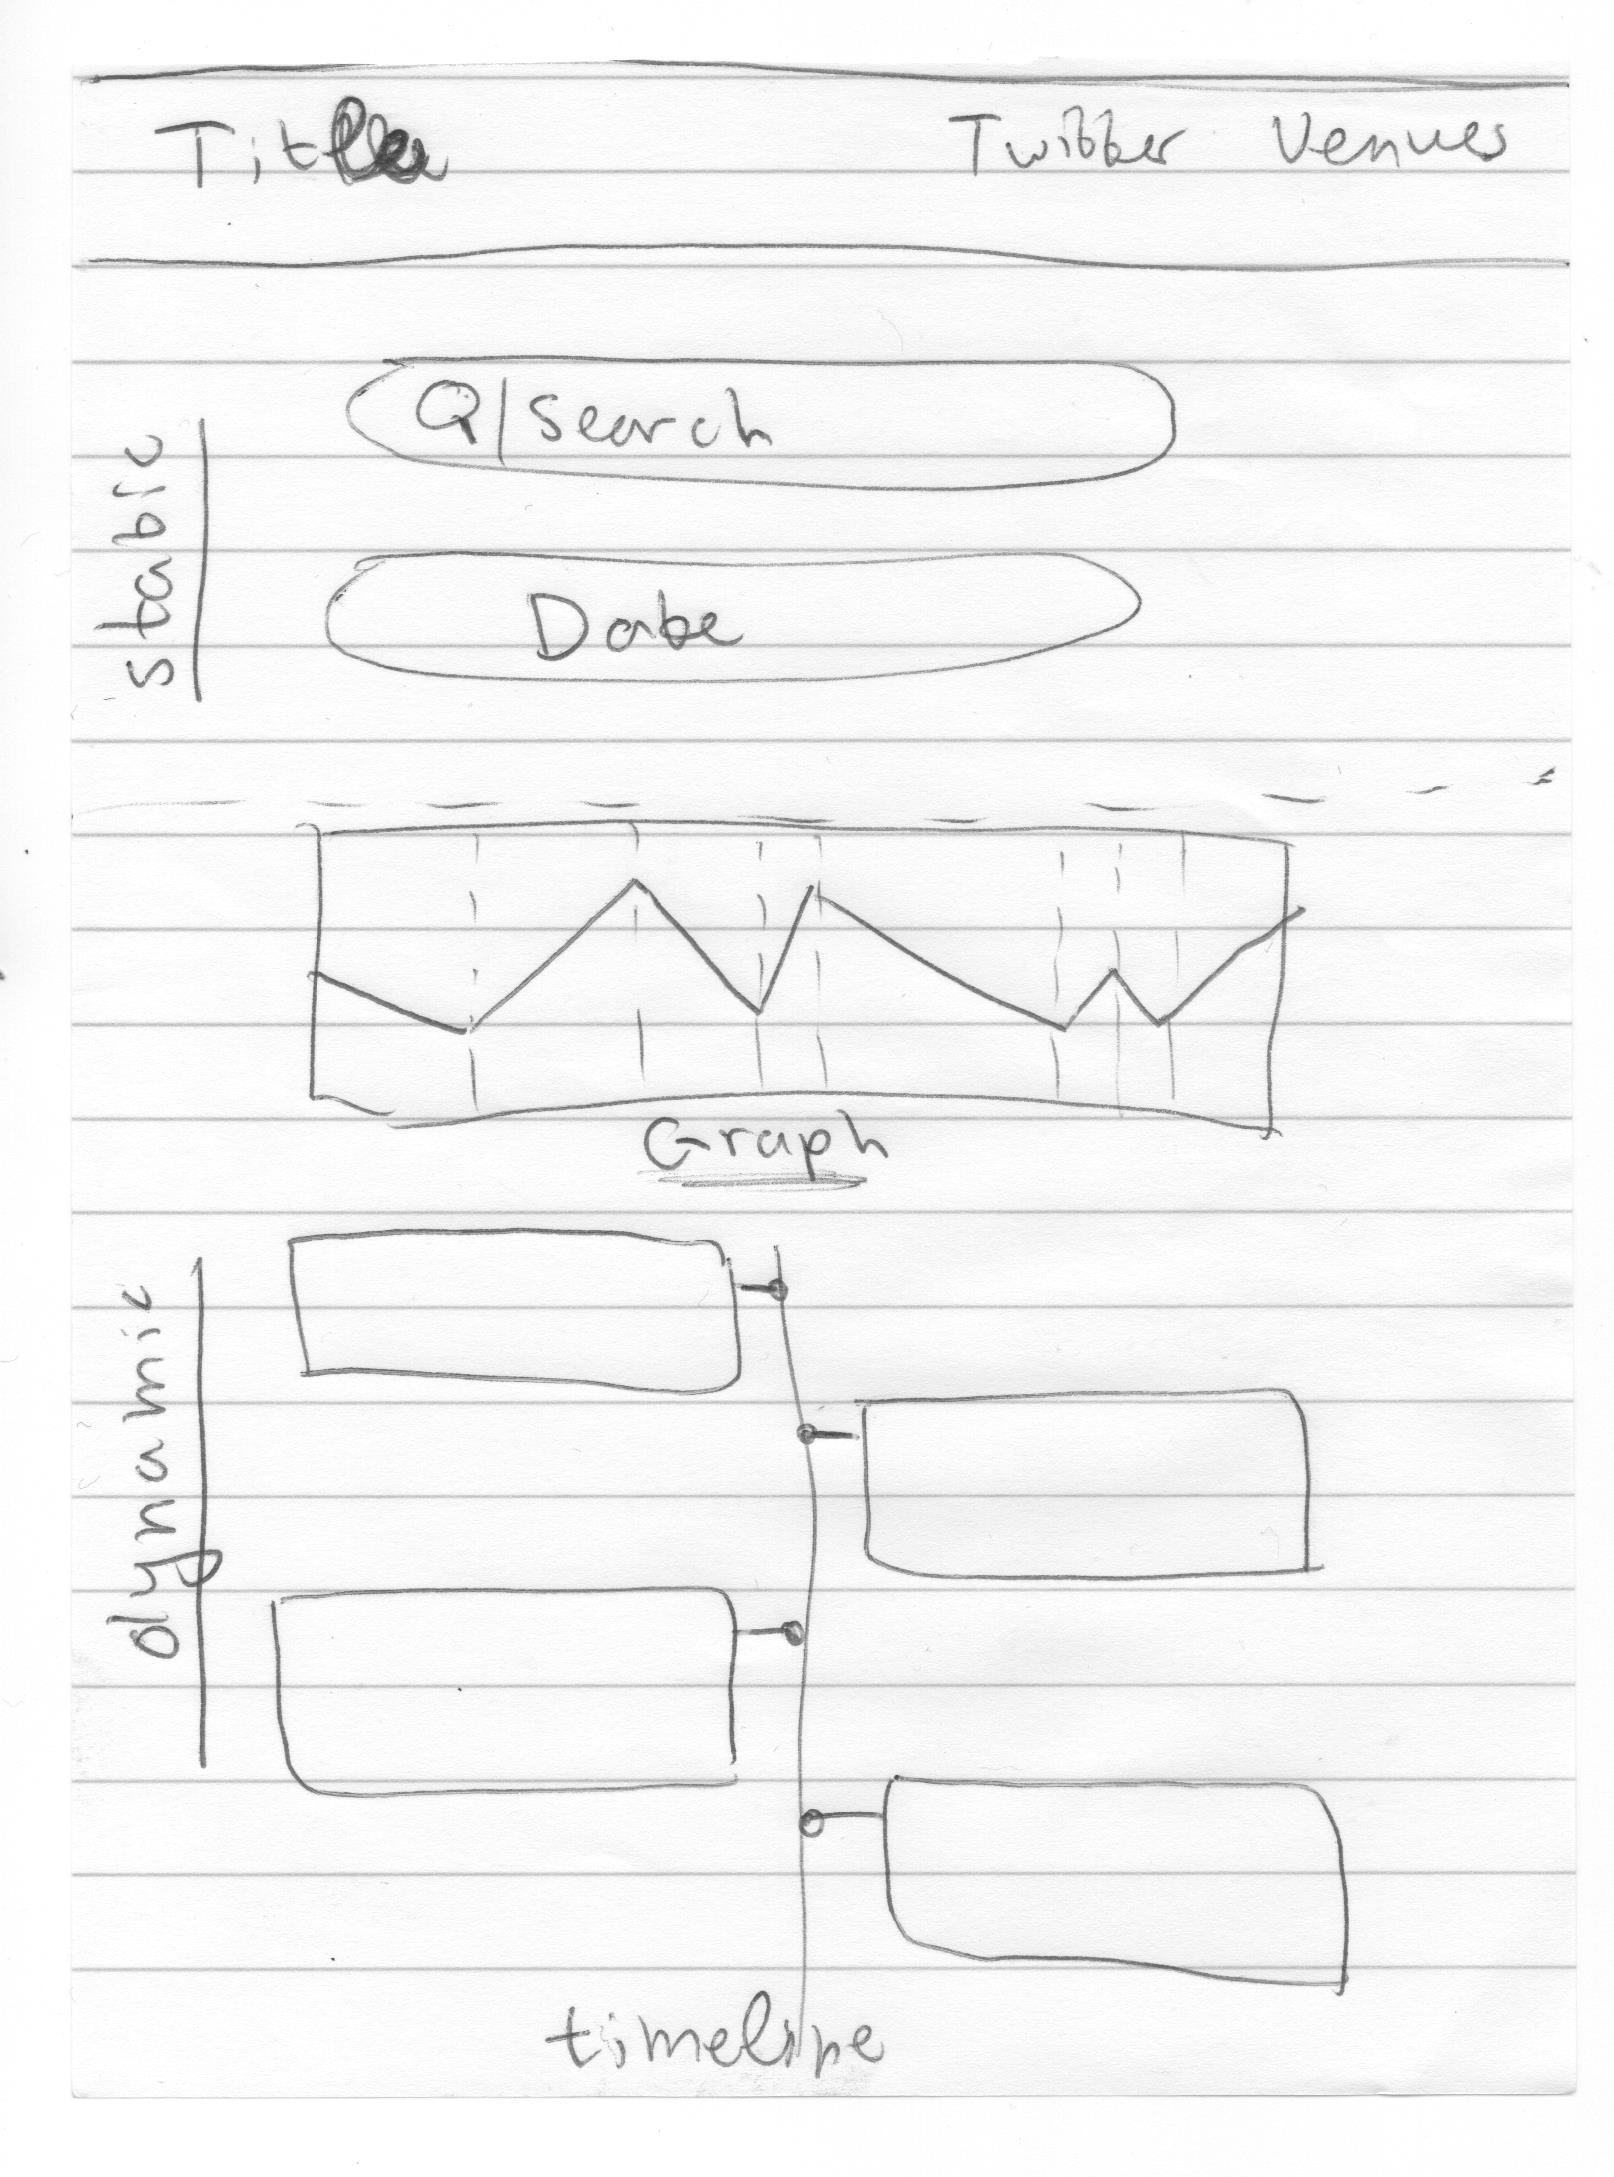
\includegraphics[width=\textwidth]{images/initialPaperPrototype}
		\caption{Initial Paper Prototype.}
		\label{initialPaperPrototype}
	\end{subfigure}
	\begin{subfigure}{.33\textwidth}
		\centering
		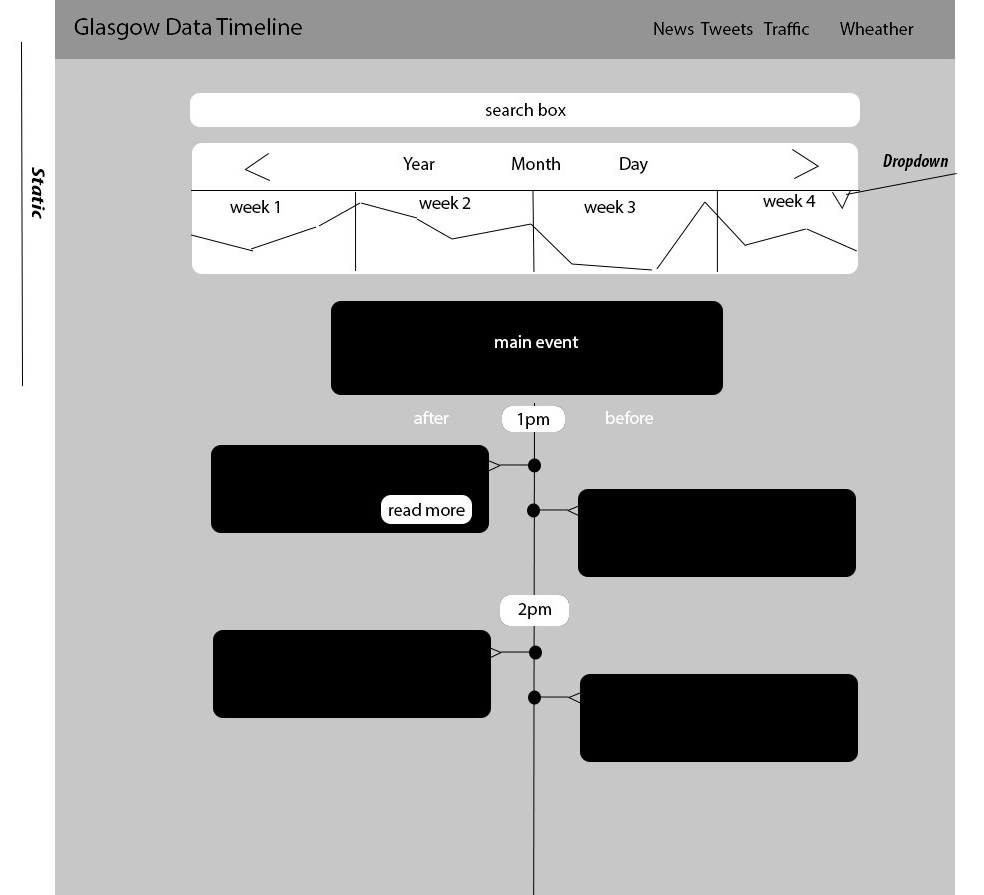
\includegraphics[width=\textwidth]{images/initialWireframe}
		\caption{Wireframe from the paper prototype}
		\label{initialWireframe}
	\end{subfigure}
	\caption{Paper Prototypes}
\end{figure} 


\paragraph{}
During the implementation process, there had been a few changes to the design. The first few iterations were enough to visualise the initial prototype and it was time to think about what the user was going to extract from using the system. Key limitations of the design were identified as it narrowed the user experience by not providing visual representation of data, that was otherwise available for use to the system. Figures  \ref{finalPrototypeEvent} and \ref{finalPrototypeCompare} show the new version of the design. A map component was included so any service, that uses location based input can be used. Also a Comparison Screen(Figure: \ref{finalPrototypeCompare}) was designed so that users will be given the opportunity to compare events side by side. The list of requirements and user stories was updated to reflect on these changes.

\begin{figure}[H]
%		\begin{subfigure}{.33\textwidth}
%			\centering
%			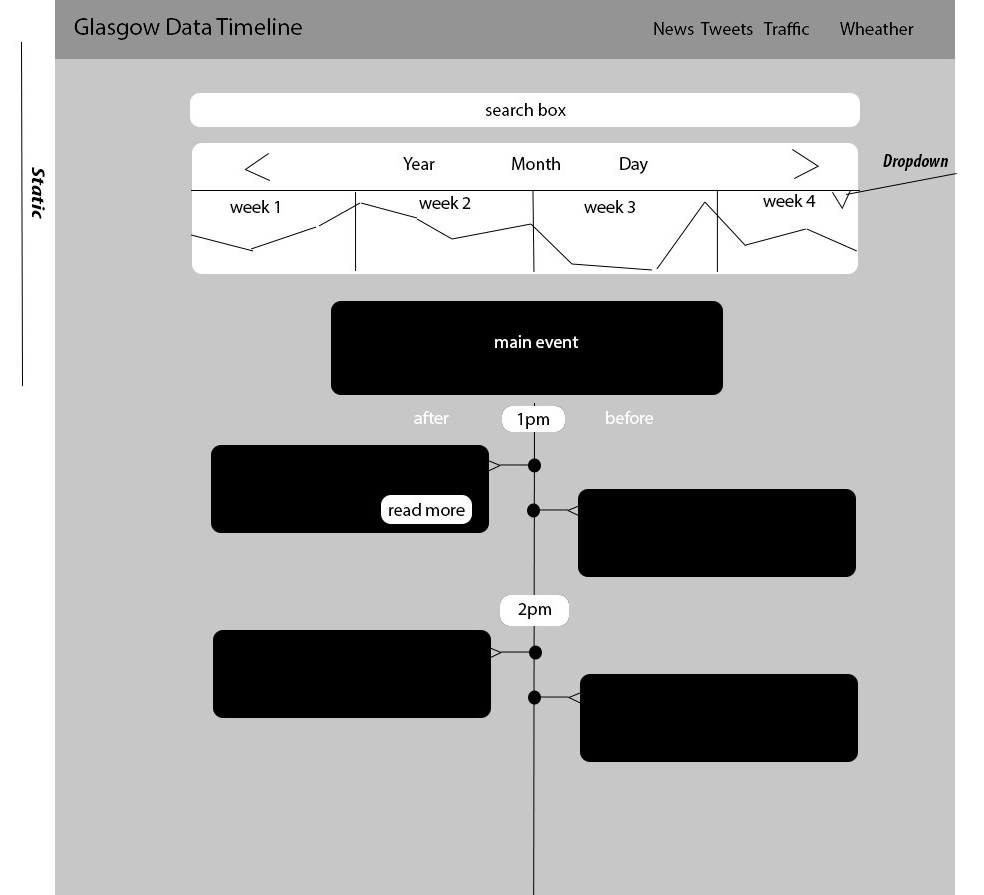
\includegraphics[width=\textwidth]{images/initialWireframe}
%			\caption{Wireframe from the paper prototype}
%			\label{initialWireframe}
%		\end{subfigure}
		\begin{subfigure}{.5\textwidth}
			\centering
			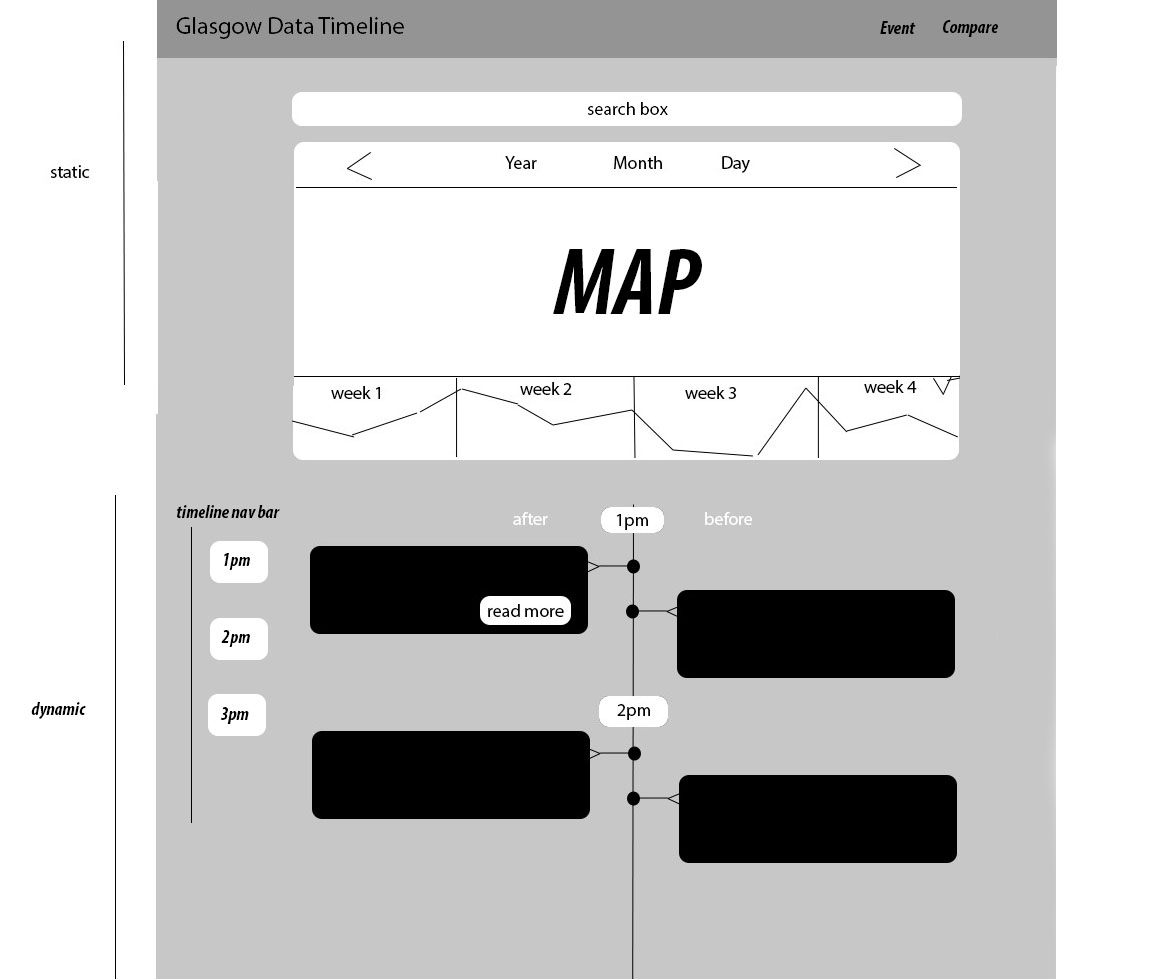
\includegraphics[width=\textwidth]{images/FinalPrototypeEvent}
			\caption{Wireframe for event exploring}
			\label{finalPrototypeEvent}
		\end{subfigure}
		\begin{subfigure}{.5\textwidth}
			\centering
			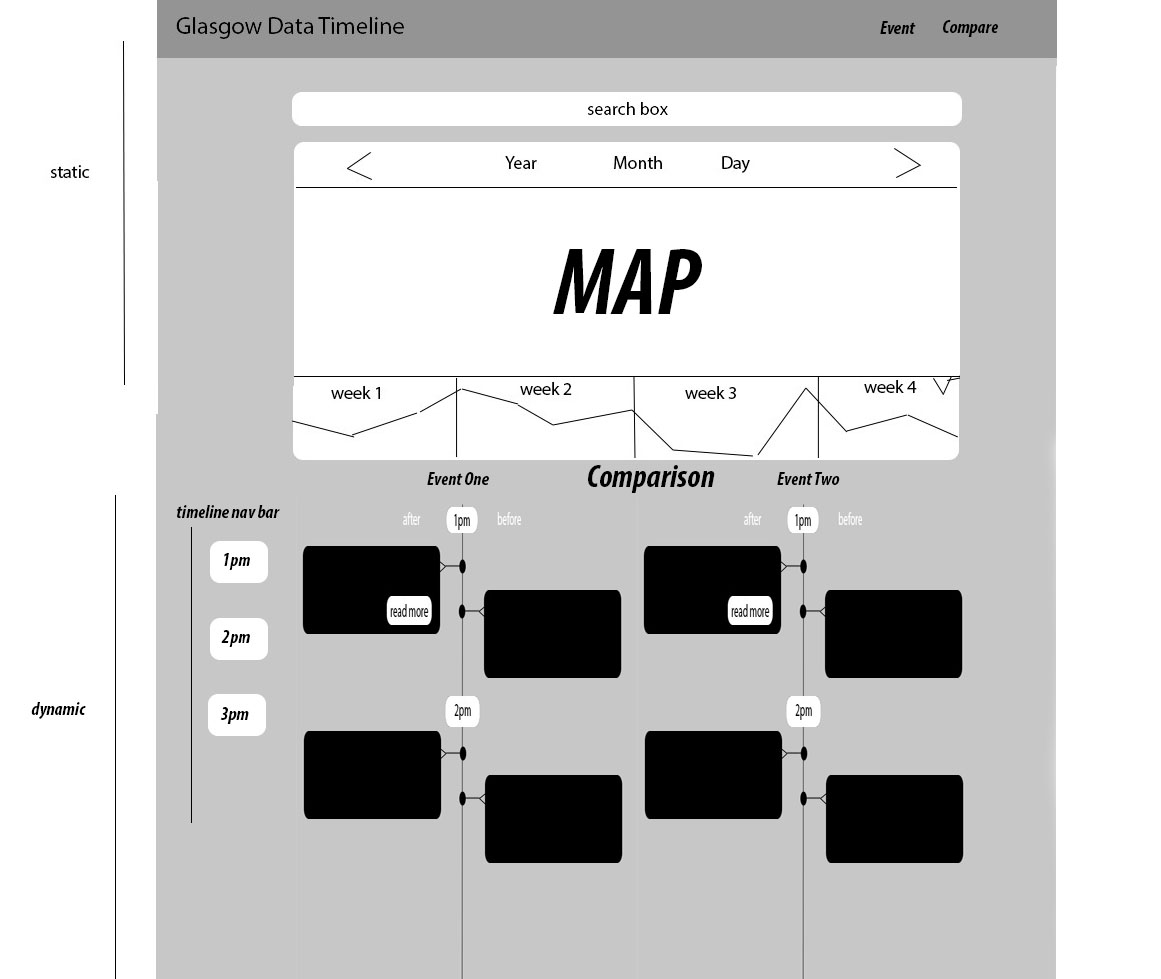
\includegraphics[width=\textwidth]{images/FinalPrototypeCompare}
			\caption{Wireframe for comparing events}
			\label{finalPrototypeCompare}
		\end{subfigure}
		\caption{Wireframes}
\end{figure}

\section{Architecture diagrams}
\paragraph{}
The Urban Data Timeline makes use of the Three Tier Architectural model as described in Section \ref{sec:highLevelDiagram}. Based on the diagram \ref{highLevelDiagram} a more in-depth diagram was designed to outline some of the key components of the system (Figure: \ref{componentDiagram}).

\subsubsection{Client}
\paragraph{}
The Client consists of the users and either a mobile device or a desktop PC. The users are going to access the application from the browser, running on their device. The browser talks to both the Google Charts API and Google Maps API, so that it can render the map and the chart, that appear in the wireframes(Figures: \ref{finalPrototypeEvent} and \ref{finalPrototypeCompare}). On the other hand, it talks to the Middleware, or in this case, the Controller component in order to get the information,  required by the user.

\subsubsection{Middleware}
\paragraph{}
The Middleware consists of four components - Controller, View, Cache, and Model. The Controller talks to all of the other components. First of all, the required data is obtained by either the Cache or the Model. If the data is not in the Cache, the Model tries to get it from the external sources. If the communication was successful, the data is stored in the Cache and returned to the Controller. From there, the Controller sends that data to the View so that the page can be prepared and returned to the user. 

\subsubsection{Data}
\paragraph{}
The Data currently consists of two services. The first one is the UBDC web service and it is key to this project as it separates into Twitter, Busy Venue, Delayed Transport, Train and Weather services(brief description of the services can be found at Section \ref{sec:aims} and \ref{subsubsec:conclusion}). As for now, only the first four services are used. The second one is the Twitter API. It is used to compensate for the limitation of the Twitter service, provided by the UBDC, which only allows for queering the results based on hash-tags. The additional API will broaden the possibilities of tweets querying by adding the option to search by username and get access to tweets from specific twitter account.        
  

\begin{figure}[H]
	\centering
	\includegraphics[width=\linewidth]{images/ArchitectureDiagram}
	\caption{Component level architecture diagram.}
	\label{componentDiagram}
\end{figure}

\section{Components communication}
\paragraph{}
This section describes how actually the components are communicating between each other. There are two scenarios, based on what request is made by the browser. 

\subsection{HTTP Request}
\label{sec:http}
\paragraph{}
The first one(Figure: \ref{HTTPRequest}) follows the traditional pattern when a user wants to access a page, which visualises data, using the application. Taking as an example one of the user stories from Section \ref{sec:userstories}, a researcher is on the home page and wants to know what are the popular tags for a given day. First step is to fill all the required inputs and then press on the search button. Then a new page is rendered on the screen and the researcher can start interacting. However, for all this to happen, the browser has to communicate with the application's server. To begin with, it makes a HTTP GET request to the controller, that maps to the action, triggered by the search button. Then all the inputs are validated against a set of rules and analysed so that the right Model can be invoked. Then the data is requested from the Model. The Model checks the Cache to see if the data is available there and if yes, returns it to the Controller. On the other hand, if the data is not available, a XMLHTTP POST Request is made to a specific Web Service and a XMLHTTP Response is received in the form of a Json object. Depending on the initial request by the researcher, some of the data from the Json is filtered out and the rest is stored in the Cache for a specified amount of time. Cache is not only part of the requirements but it is important as users, like researchers, are expected to do many similar requests by changing only one or two variables at a time. Once the model has finished, manipulating the data, it is sent back to the Controller that redirects it to the View. The View formats the data, according to its type, and sends it back to the Controller. Finally the Controller returns an HTTP Response with the generated HTML.  

\begin{figure}[H]
	\centering
	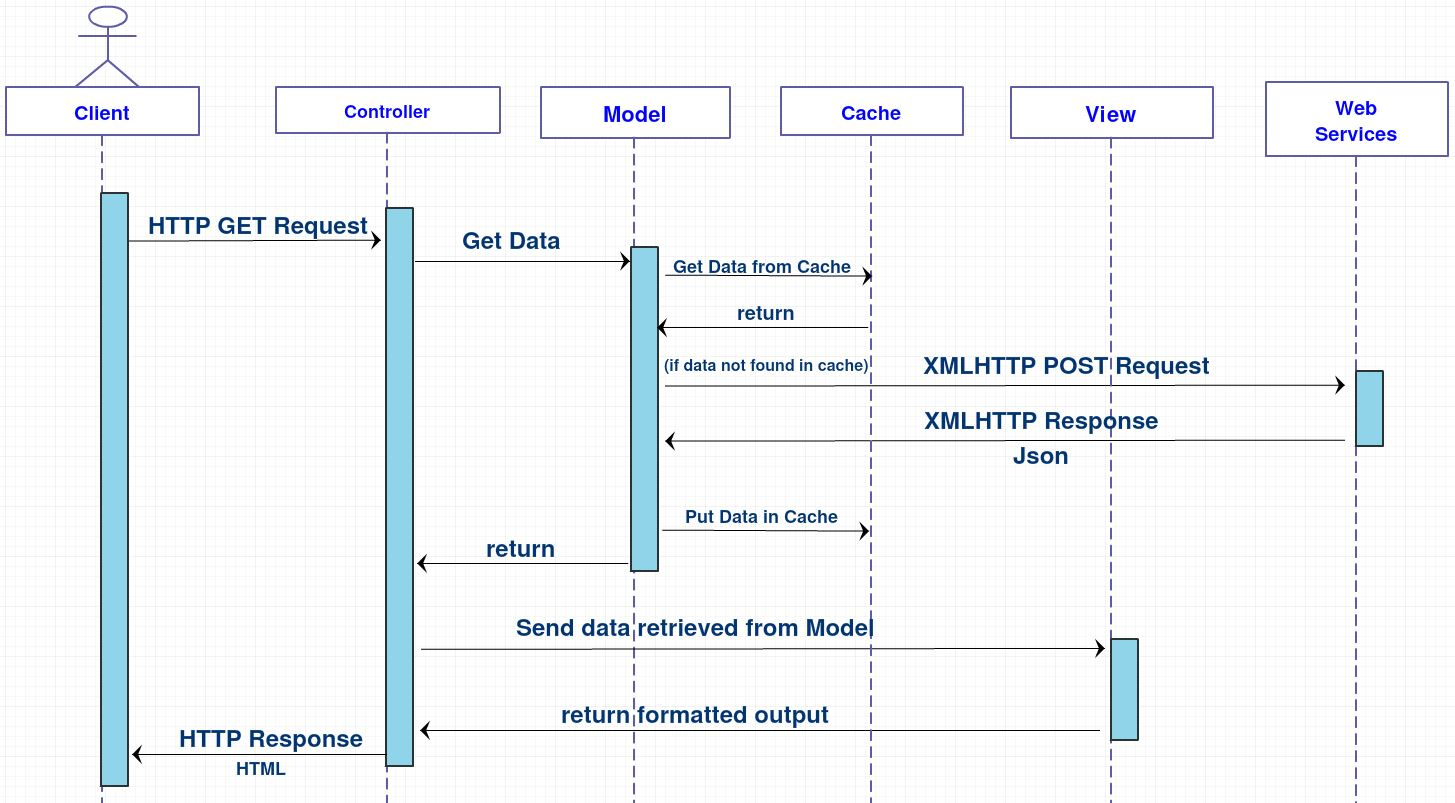
\includegraphics[width=\textwidth]{images/HTTPRequestSequenceDiagram}
	\caption{HTTP Request Sequence diagram}
	\label{HTTPRequest}
\end{figure}

\subsection{XMLHTTP Request}
\label{sec:xmlhttp}
Following from the requirements(Section: \ref{sec:functional-requirements}) and the paper prototypes(Section: \ref{sec:paper-prototypes}), some of the elements(Map and Chart) can be rendered by the View but in order to make them responsive, these elements have to use Ajax in order to be populated. Taking as an example one of the user stories from Section \ref{sec:userstories}, a restaurant owner wants to view venues that are nearby but also may want to get the same information but for a place, which is not the same as his current location. In order not to reload the page every time, Ajax performs XMLHTTP Requests instead of HTTP Request and the received response will be used to update the page dynamically. In order to handle such requests, the system must provide REST endpoints that are compatible. If the browser makes a XMLHTTP request(Figure: \ref{XMLHTTPRequest}) to one of the endpoints, the Controller, similar to the previous case, performs the same steps but in this case there is no communication with the View. The data, returned from the services, is filtered and sent, via a XMLHTTP Response in a Json format, back to the client. 

\begin{figure}[H]
	\centering
	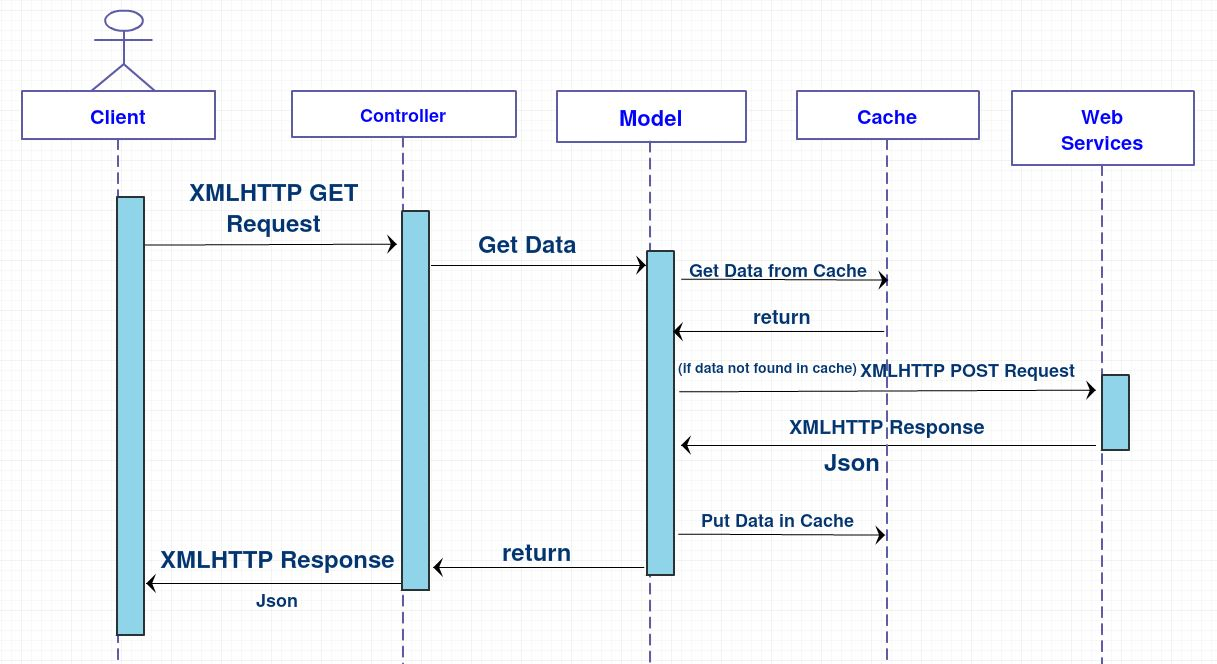
\includegraphics[width=\textwidth]{images/XMLHTTPRequestSequenceDiagram}
	\caption{XMLHTTP Request Sequence diagram}
	\label{XMLHTTPRequest}
\end{figure}

\section{Choice of technology}
\label{sec:choiceoftec}
\paragraph{}
One of the requirements (Section: \ref{tab:nonFuncReq}) states that the application should be accessible and compatible with desktops, laptops, tablets and smartphone devices. This limits the options in terms of platforms that can be used. A common tool for all these devices is the web browser. For desktops and laptops, this is a great choice as there is a big variety of browsers. On the other hand, this introduces another challenge to the development as some technologies are not compatible with some older browsers like Internet Explorer 7 or lower. Additionally, native applications, developed specificity for a mobile platform like Android or iOS tend to perform better than their web alternatives but will take longer to implement so they are not suitable for such project. This section will present technologies, which will fulfil the requirements.

\subsection{Security}
\paragraph{}
Security is top priority when developing a web application. As this project will be used only for displaying data, there are not many vulnerabilities that can be targeted by attackers. First of all, the system will not make use of a database so any attempts for performing SQL Injection, Cross-Site Request Forgery, Sensitive Data Exposure or Cross Site Scripting (XSS) will not lead to a security breach. However, as a safety precaution, all inputs that are received must be validated before being passed to any of the external services shown in Figure \ref{componentDiagram}. Furthermore, the application will not require authentication so it is not vulnerable to Insecure Direct Object References or Broken Authentication via stolen cookies. The only possible vulnerabilities are Denial of Service and Man in the middle attacks. For this project, no defence mechanisms will be developed against these attacks. The first one can be mitigated by following the web traffic and blocking suspicious requests. The result of a successful Denial of Service attack will be that users will not be able to access the system due to the server, on which the application is running, has be overloaded with requests and is not able to respond. Man in the middle is a form of attack where the user's network has been breached and an attacker is modifying their traffic. The way to defend against this attack is by introducing the HTTPS protocol that ensures the uniqueness of a website but it requires an expensive certificate. However, all of the following technologies have to be compatible with the HTTPS protocol in case that it is decided to be included in a future iteration.   

\subsection{Web Application Framework}

\subsubsection{Play Framework}
\paragraph{}
Play Framework 2\footnote{\url{https://www.playframework.com}} is is an open source web application framework, written in Scala and Java, which follows the model–view–controller (mvc) architectural pattern. 
\\ \textbf{Pros}:
\begin{itemize}

\item It dramatically improves the productivity of a developer compared to other Java based web frameworks like Jersey or Spring MVC. The server does not have to be restarted manually in order to see the changes. \textit{Hot reload} is available for all Java classes, templates and configurations allows for much rapid development. This is available in many dynamic languages, but it is not provided in any other Java framework.

\item Play 2 is open source. If required, everything can be seen how it works. It has a relatively large community, represented by questions on StackOverflow and developers that contribute with developing plug-ins.

\item Java: type safe language. Also JVM performs great and can scale to support many developers and users. Furthermore, Java by itself has a large community and 
wide variety of IDEs\footnote{Integrated Development Environment} and available libraries.
	
\end{itemize}
\textbf{Cons}:
\begin{itemize}
\item Play 2 is a relatively new framework so the community is not as big compared to other Java frameworks. 

\item The framework is immature. Good practises are still no clearly defined. 

\item Java does not provide features like closures to keep asynchronous code clean. Play is built on top of asynchronous input and output. There are ways to go around this but the application will end up with lots of inner anonymous classes, which will reduce the maintainability and readability of the code.

\item Java does not support Json natively so a third-party library must be used. This, together with its strict types, will lead to big overheads when parsing Json, which 
is going to be the main source of data for this project.  
\end{itemize}

\subsubsection{Django}
\paragraph{}
Django\footnote{\url{https://www.djangoproject.com}} is free and open source web application framework, written in Python. Its main focus is helping developers to write code, without the need to reinvent the wheel.
\\ \textbf{Pros:}
\begin{itemize}
	\item Django follows the DRY principle: Do not Repeat Yourself. The frameworks is designed so that developers can get the most out of a little piece of code. In addition, this automatically leads to less hours spent in developing and a lower chance of introducing bugs.
	\item Good documentation. Django provides sufficient documentation for every release with plenty of code examples. Furthermore, if something is not documented, the code is publicly available on GitHub so 
	it can be directly inspected from there or from an IDE like PyCharm. 
	\item Django provides build-in Admin panel, that is generated automatically for each project. It allows users to manipulate and control users or database objects, specific to the application.
	\item Django is scalable as it is designed on a component based architecture. All the components are decoupled and does not depend on each other so they can be easily unplugged and replaces. Likewise, new components can be simple to introduce. 
	\item Django provides a set of tools that can be useful when writing tests. Tests can be perform not only on the Models and the Controllers, but also on the Views without a third-party library. It provides a build-in request factory, which uses URL resolution to trigger the views. 
\end{itemize}
\textbf{Cons:}
\begin{itemize}
	\item Django is using Python, that is an interpreted language, and it is often slower than compiled languages.  
	% \item If the application is using a database, long queries that make use of multiple JOINs or UNIONs can be quite hard to implement.  
\end{itemize}
\subsubsection{Laravel}
\paragraph{}
Laravel\footnote{\url{https://laravel.com}} is a free, open-source PHP web framework, intended for the development of web applications following the model–view–controller (MVC) architectural pattern.
\\ \textbf{Pros}:
\begin{itemize}
	\item Composer - packaging system for PHP and is used for dependency management. Laravel is designed using a component based architecture and the whole framework is available as individual Composer packages. 
	\item Blade is the Laravel's template engine that is lightweight and provides clean syntax for views. It supports template inheritance that reduces the duplication of code and re-usability of specific template components. 
	\item Resourceful controllers: generic routes can be made that directly map to resources in the controller. Makes developing REST a bit easier.
	\item Laravel is built with testing in mind. It supports PHPUnit directly out of the box. Same as with Django, it provides helper methods that allows for expressive testing.  
	% \item Community is great with many active people on the Laravel's forums.
	\item Error messages are easy to understand and points directly to the error.
	\item PHP has built in Json support.
\end{itemize}
\textbf{Cons}:
\begin{itemize}
	\item PHP: inconsistent function names in the standard library(for example: isset() and isnull())
	\item Same as with Python, PHP is an interpreted language so that it is slower than compiled languages. However, PHP 7 is advertised to have a big performance improvement over PHP 5.
\end{itemize}

\subsubsection{Choice}
\paragraph{}
Laravel was chosen for this project. It is very similar to Django and offers the same features. In addition, PHP 5 and Python are both interpreted languages with similar performance and have built in Json support. However, updating in a future iteration to PHP 7 with its improved performance and speed, twice as fast as PHP 5.6\footnote{\url{http://php.net/releases/7_0_0.php}}, will reduce the computation time that is taken by sorting and filtering the data from the services. Finally, Laravel is compatible with HTTPS requests and will allow for a future security update. On the other hand, Play Framework 2 is not suitable for this project as it urges on using Java, which will bring a big overhead when processing Json objects. 


% http://www.codeproject.com/Articles/1044334/jQuery-Vs-AngularJS-A-Good-Comparison
\subsection{Javascript Library}
\paragraph{}
In order to improve the user experience and embed a chart and a map into the design, an asynchronous Javascript library is required to simplify the calls to the REST endpoints. Two options were researched: jQuery and AngularJS.
\\\hspace*{7mm}\textbf{jQuery}\footnote{\url{https://jquery.com}} is a lightweight Javascript library, which comes with many features. It broadly simplifies the use of Javascript for client-side scripting. It can:
\begin{multicols}{2}
	\begin{itemize}
		\item manipulate the content of a web page.
		\item make use of built in effects and animations.
		\item easily make Ajax requests.
		\item traverse though the DOM.
	\end{itemize} 
\end{multicols}
\textbf{AngularJS}\footnote{\url{https://angularjs.org}} is a MVC framework, developed by Google. Compared to jQuery it has more features but being a framework emphasis on following its rules. It can:
\begin{multicols}{2}
	\begin{itemize}
		\item make use of templates.
		\item validate forms.
		\item perform Ajax requests.
		\item be tested.
	\end{itemize} 
\end{multicols}

\subsubsection{Choice}
JQuery was chosen for this project as it is a fast and feature-rich Javascript Library. It allows for more flexibility in the implementation as it is not a framework like AngularJS. 

\subsection{CSS Framework}
\paragraph{}
With the rise of mobile devices, making responsive websites and keeping up with the latest technologies is very time consuming and hard to maintain. There are many CSS frameworks that solve these problems but Bootstrap\footnote{\url{http://getbootstrap.com}} and Skeleton\footnote{\url{http://getskeleton.com}} were the one compared for this project. They both are very simple to get started with: just reference the framework into the header of the page. Both offer 12 column grid system as well as many layouts and components. One of the most important features, that is offered by both frameworks, is providing responsive utility classes that can automatically rearrange a page based on the screen size of the device. However, Bootstrap was the one, chosen for this project as, first of all, it has the best documentation. Bootstrap also comes with Javascript plug-ins like drop downs, tool-tips, pop-ups, sliders and many more.   

%https://www.quora.com/How-does-D3-js-compare-with-Google-Charts-API
\subsection{Graph API}
\paragraph{}
Following from the requirements(Section: \ref{sec:functional-requirements}), the application should provide graph visualisation. For this purpose, two APIs were considered: D3.js and Google Charts.  
\\\hspace*{7mm}\textbf{Google Charts}\footnote{\url{https://developers.google.com/chart/}}:
\begin{multicols}{2}
	\begin{itemize}[noitemsep]
		\item contains a wide varsity of charts.
		\item has a great documentation.
		\item offers fully implemented examples for all charts. 
		\item provides extra features like exporting charts as images.
	\end{itemize} 
\end{multicols}
\textbf{D3.js}\footnote{\url{https://d3js.org}}:
\begin{multicols}{2}
	\begin{itemize}[noitemsep]
		\item offers flexibility.
		\item does not have a limit on how much data to display.
		\item provides extra features like zooming and clicking.
		\item can be used for creating very complex graphs.
	\end{itemize} 
\end{multicols}
\subsubsection{Choice}
Google Charts Graph API was chosen for this project due to its simplicity and great documentation. Furthermore, there is no intention of building big and complex graphs in the time, allocated for this project.  

\subsection{Map API}
\paragraph{}
Going back to the requirements (Section: \ref{sec:functional-requirements}) and the paper prototypes(Section: \ref{sec:paper-prototypes}), the application must be able to show venues on a map and also to take location based input. To simplify the implementation, it will be useful to find an API that provides functionality to fulfil both requirements. Google Maps API\footnote{\url{https://developers.google.com/maps/}} was chosen for this project as it is the only one that is free and has built it support for all the required features. In addition, it offers 25,000 map loads per 24 hours for 90 days\cite{mapusage}. It also provides wide variety of customisable options like colours, shapes, markers and many more. Furthermore, Google Places\cite{mapplace}, part of the Google Maps API, features more than 100 million businesses and points of interest that are updated frequently through owner-verified listings and user-moderated contributions. It gives the ability to search for specific place and can be configured to display details like ratings and reviews.

\section{Summary}
Finally, this chapter outlines the details, needed before the start of the implementation. It shows how the system is supposed to look like, both in terms of the interface and the component structure. Furthermore, it lists the technologies that were used for the implementation. On the other hand, the next chapter highlights some of the main steps and challenges that were identified during the iterations, allocated for developing a prototype and transforming it to a final product.    

\chapter{Implementation}
\section{Prototype Implementation}
\paragraph{}
The first three iterations of the project focused on the background research, project planning, requirements gathering and choosing the technologies. Furthermore, the fourth iteration involved producing a prototype out of the wireframes(Figure: \ref{initialWireframe}). A simple static HTML page was developed to represent the key components: search box, date picker, chart and timeline. The search box(Figure: 5.1) was a simple input html field. Its purpose was to get the required tweet hash-tag. Also a hint was included(\textit{input a query}) in order to make it clear what this field was supposed to take as parameters. The date picker was implemented using dropdown menus for the day, the month and the year. Two additional buttons were added on both sides to help the user to quickly adjust the date input without the need to go and use the menus again.        

\begin{figure}[H]
	\centering
	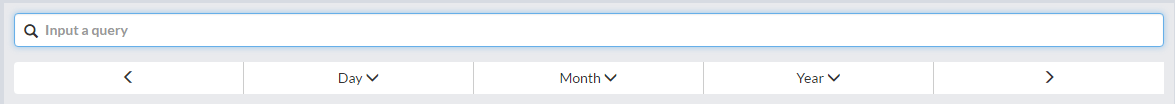
\includegraphics[width=\textwidth]{images/searchboxwithdatepicker}
	\label{fig:searchbox}
	\caption{Search Box and Date picker}
\end{figure}

\paragraph{}
For the purpose of the prototype, an open-source vertical timeline was used. It was implemented using jQuery and CSS3, which perfectly suited the technologies(Section: \ref{sec:choiceoftec}), used for this project. With its responsiveness and clear design, it was a perfect choice for representing the initial outline of the interface. During this iteration, no back-end logic was introduced, as main focus was evaluating and finalising the design before the start of the next iteration. 

\begin{figure}[H]
	\centering
	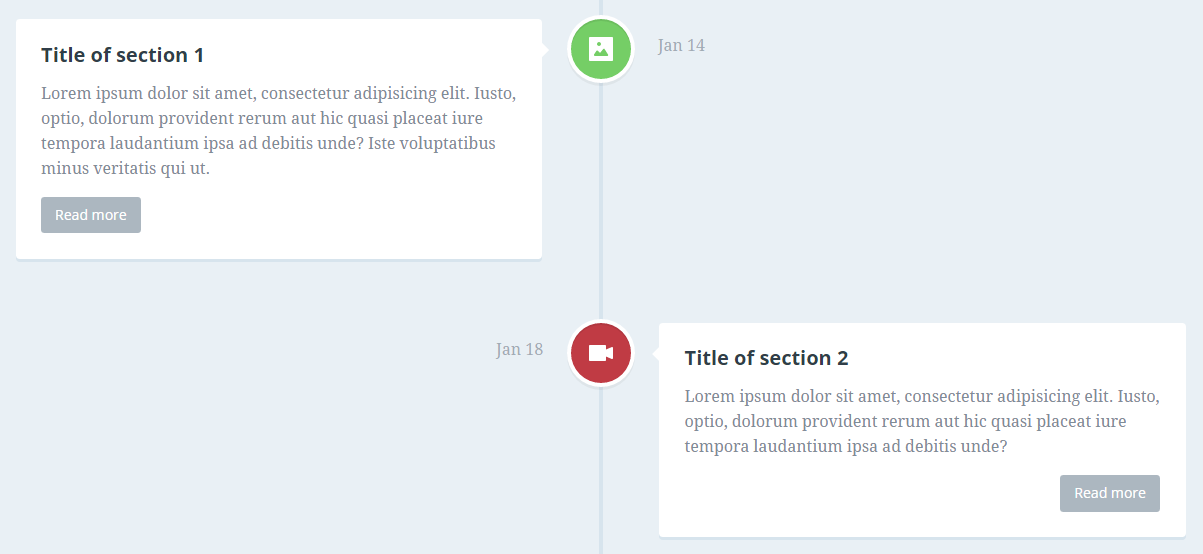
\includegraphics[width=.5\textwidth]{images/opensourcetimeline}
	\label{fig:opensourcetimeline}
	\caption{Initial timeline}
\end{figure}

\section{Product Implementation}
\paragraph{}
Accordingly, during the fifth iteration, the prototype was re-factored to make use of a Model-View-Controller framework, which was chosen in Section \ref{sec:choiceoftec} so that communication with the services could be introduced.

\subsection{Model}
\label{sub:model}
\paragraph{}
The models represented the data. They, as shown on the architecture diagram(Figure: \ref{componentDiagram}), corresponded to an external service. At the start, in order to learn how the framework worked, each model was implemented separately. However, this led to a lot of repetitive code so another approach was considered. As PHP supported Object-Oriented programming, the common features from all the models were extracted and an Abstract class was implemented. 
\begin{lstlisting}
abstract class AbstractService
{
	/** holds the service url*/
	protected $url;
	
	/** holds the input query*/
	protected $query;
	
	/** holds the request parameters*/
	protected $postData;
	
	/** holds the input date*/
	public $queryDate;
	
	/** holds the response from the services*/
	public $response;
	
	abstract public function getCount();
	
	abstract public function getData();
	
	public function sendRequest($arrayToSend)  
}  
\end{lstlisting}
\paragraph{}
Using the abstract class mentioned above made including another service really easy. The public method \textit{sendRequest} was common for all models as it was used for communication with the services. The parameter, that it took, \textit{\$arraytoSend} represented the array of parameters, that the service required as inputs. The methods \textit{getCount()} and \textit{getData()} were implemented in each Model accordingly. The idea behind them was to process, filter and format the response from a service and return either the count or an array of entries, that the user had required.  

\paragraph{}
In addition, the Busy Venues service was returning information about the venues, which in some cases included the venue's twitter account. However, the Twitter service did not allow searching for tweets, based on user's account. In order to compensate for this limitation and increase the amount of data sources, it was decided to include communication with the genuine Twitter API as shown on the architecture diagram(Figure: \ref{componentDiagram}). With Laravel's flexible design and high separation of concerns, it was possible to integrate an additional component that would perform the required communication. Thujohn/twitter\footnote{https://packagist.org/packages/thujohn/twitter} was a php component that was able to be integrated with Laravel and allowed for extracting a collection of the most recent Tweets, posted by specific user. It allowed for searching based on screen\_name or user\_id. The only requirement for it to work was creating a Twitter account and enabling the API by generating the appropriate keys and tokens. 
\begin{lstlisting}
return Twitter::getUserTimeline(['screen_name' => 'thujohn', 'count' => 20, 'format' => 'json']);
\end{lstlisting}

\subsubsection{Challenges}
\paragraph{}
At the beginning of the project, the services were still under development. A few problems were identified at the beginning of the implementation. First of all, the Twitter service was not returning a time-stamp for each tweet. As a timeline was built, the time was a key factor. To go around this issues, until the services were fixed, a random time generator was developed so that the tweets can be listed on the timeline. Furthermore, the Busy Venue service was behaving not as expected as some venues, despite the fact that they were returned with score higher than 0, they did not seem to have any entries (all entries were set to 0). On the other hand, some venues with score 0 had entries greater than 0. Again, another random generator, in this case generating attendance, was introduced so that venues could be visualised on the timeline. 
\paragraph{}
Consequently, after introducing the communication with Twitter, registering to use the API for free came with some limitations. Twitter restricted the usage to 180 requests in 15 minutes and advised the developers to cache the responses locally. As Laravel supports caching, it was decided to implement this extra functionality and use file system cache in order not to fill up the memory of the server, as well as, not to increase the overhead of the project by designing and introducing a database. The Caching capabilities of Laravel were very flexible and allowed for directly inserting objects and specifying a time limit for how long each insertion stayed in the Cache. 
\begin{lstlisting}
    public function sendRequest($username)
	    {
	    $user = $username;
	    $cacheTag = 'twitterTimeline'; //config timeline twitter
	    $cacheKey = $user . "-" . $cacheTag;
	    $cacheLimit = 15;
	    $tweets = null;
	    
	    /* caching */
	    if (Cache::has($cacheKey)) {
		    $tweets = Cache::get($cacheKey);
	    } else {
		    $tweets = Twitter::getUserTimeline(['screen_name' => $user, 'count' => 10, 'format' => 'object']);
		    Cache::put($cacheKey, $tweets, $cacheLimit);
	    }
	    return $tweets;
    }
\end{lstlisting}
\paragraph{}
In addition, Caching was a part of the requirements(Table: \ref{tab:funcReq}). As it is shown on the architecture diagram(Figure: \ref{componentDiagram}), it was included for all the Models as most of the users were expected to be researchers, who would not perform random queries but rather adjust some of the input parameters to extract the most out of the system. As a result, when a request was made, there would be no point in requesting data, needed for a previous search. Furthermore, this resulted in a reduced number of the requests to the external services. 


\subsection{View}
\label{sub:view}
\paragraph{}
The views represented an interface to present the data from the models as shown on the HTTP sequence diagram(Figure: \ref{HTTPRequest}). Initially, they were static pages. However, after migrating to the MVC pattern, using Laravel, the project benefited from the template engine, which the framework provided, called Blade\footnote{https://laravel.com/docs/5.1/blade}.Two of the primary benefits of using Blade were template inheritance and sections. Since this project maintained the same general layout across all views, it was convenient to define it in a single Blade template, which was extended by all the pages:
\begin{lstlisting}
	<!DOCTYPE html>
	<html lang="en">
	<head>
		<meta charset="utf-8">
		<meta http-equiv="X-UA-Compatible" content="IE=edge">
		<meta name="viewport" content="width=device-width, initial-scale=1">
		@yield('title')
		@include('layout.style')
	</head>
	<body>
		@include('templates.partials.navigation')
	
		@yield('content')
		
		@include('layout.script')
	</body>
	</html>
\end{lstlisting}
\paragraph{}
This file contains typical HTML mark-up. However, it makes use of the @include and @yield directives. The @include directive defined a feature or component from the interface, while the @yield directive was used to display the contents of a given section, taken from a child page. This structure allowed for high flexibility as well as modularity. 

\paragraph{}
One of the requirements was about visualising data on a graph(Table: \ref{tab:funcReq}). Accordingly, a chart view component was introduced. Initially, a bar chart was developed from scratch. However, due to time constraints, an already implemented solution was introduced, which offered a lot more extra features and ensured compatibility with different browsers. Google Charts was very flexible as it was adjusting the graph, based on the input that was given. For example, when the input was an array of arrays of length 2: \textit{[['2014-08-21',10],['2014-08-22',20]..]}, a single bar for each data was presented(Figure: \ref{singlechartsmall}). On the other hand, when the input was \textit{[['2014-08-21',10,15],['2014-08-22',20,11]..]}, two bars for each date with different colours were shown (Figure: \ref{comparechartsmall}). Furthermore, as the project was making use of data from different domains, each that offered some way to count events got its own chart representation. The one for the Twitter service was showing number of tweets for a given hash-tag. On the other hand, the Busy Venues service chart was presenting the number of busy venues in a specified area. The user could easily switch between charts by clicking on the buttons, labelled with the corresponding service name.

%Also made the chart to draw any number of charts passed from the Controller so if a new service is add, there will be no need to change the way the chart works.
%o HOW IT WORKS – controller returns a response in the form: {"yesscotland":{"twitter":[{"date":"2014-08-21","count":126},{"date":"2014-08-22","count":629}, … ],"venues":[{"date":"2014-08-21 12:08:00","count":7},{"date":"2014-08-22 12:08:00","count":7} …]} - client jQuery code reads this and for each key it creates a button and stores the array corresponding to that key. On button click, jQuery gets the name of the button and draw the data corresponding to that name.

\begin{figure}[H]
	\centering
	\begin{subfigure}{.3\textwidth}
%		\centering
		\includegraphics[width=.8\textwidth]{images/singleChartSmall}
		\caption{Single Chart}
		\label{singlechartsmall}
	\end{subfigure}
	\begin{subfigure}{.3\textwidth}
%		\centering
		\includegraphics[width=.8\textwidth]{images/compareChartSmall}
		\caption{Compare Chart}
		\label{comparechartsmall}
	\end{subfigure}
	\caption{Charts}
	\label{fig:chartsmall}
\end{figure}

\paragraph{}
Additionally, taking location input was one of the requirements(Table: \ref{tab:funcReq}). In order to achieve that, a map component was introduced, which made use of Google Maps API(Figure: \ref{mapsmall}). To allow the user to quickly find a place on the map, an input field was included that offered searching based on name and location(Figure: \ref{mapsearchsmall}). Furthermore, each marker contained information about the venue, which was representing(Figure: \ref{mapvenuessmall}). The map was populated with data, retrieved from the Controllers(Section: \ref{subsec:controller}) with an Ajax request. On every change of the location, a new request was made to get the nearby venues.

\begin{lstlisting}
 google.maps.event.addListener(marker, 'dragend', function (evt) {
	  map.setCenter(evt.latLng);
	  lat.value = evt.latLng.lat();
	  lng.value = evt.latLng.lng();
	  getNearbyVenues();
 });
\end{lstlisting}

\begin{figure}[H]
	\centering
	\begin{subfigure}{.3\textwidth}
		%		\centering
		\includegraphics[width=\textwidth]{images/mapsmall}
		\caption{Map}
		\label{mapsmall}
	\end{subfigure}
	\begin{subfigure}{.3\textwidth}
		%		\centering
		\includegraphics[width=\textwidth]{images/mapsearchsmall}
		\caption{Map search}
		\label{mapsearchsmall}
	\end{subfigure}
	\begin{subfigure}{.3\textwidth}
		%		\centering
		\includegraphics[width=\textwidth]{images/mapvenuesmall}
		\caption{Venue information}
		\label{mapvenuessmall}
	\end{subfigure}
	\caption{Map Component}
\end{figure}

\paragraph{}
With the extra functionality of the map, new possibilities for the user to browse different series of events were introduced. Google Maps API allowed for the markers on the map to be clicked. Part of the data, received from the Busy Venues service was about the venue's time-series. In addition, the Train Delays service was offering a time-series of train delays for a particular train station. Table \ref{tab:contentuserinput} summarises the new alternatives, presented to the users based on their input. However, due to time constraints, train delays were not included in the views. 

\begin{table}[H]
	\centering
	\begin{tabular}{|p{2cm}|p{7cm}|p{7cm}|} \hline
		&	Query	& No Query \\ \hline
		Location(click on the map) 	& Timeline of tweets with information about busy venues	in radius of half a mile.	& Timeline of busy venues around the area  \\ \hline
		Location(click on a venue)	& Timeline of tweets for the query combined with tweets for this venue and hourly information about this venue	& Venue time series – including	hourly information about the venue with tweets from the venue’s twitter account  \\ \hline
		Location(click on train station)	& Timeline of tweets for the query combined hourly information about train delays from this train station & 	Timeline of train delays \\ \hline
	\end{tabular}
	\caption{Timeline content based on user input}
	\label{tab:contentuserinput}
\end{table}


\paragraph{}
In addition, one of the \textit{Could have} requirements for the user interface(Table: \ref{tab:funcReq}) was to show a summary of the performed search, a box that pops up from the top and sticks there while scrolling was included as a component. The purpose of this box was to store key statistics and also to provide the user with other popular tweet hash-tags, based on the already provided input(Figure: \ref{zebrainfobox}).  

\begin{figure}[H]
	\centering
	\includegraphics[width=\textwidth]{images/infobox}
	\label{zebrainfobox}
	\caption{Information Box}
\end{figure}

%google maps api - progress 8
%input - we could not use the venue search from google as coordinates missmatch so a rest api was introduced
%venues search progress 12
\subsubsection{Challenges}
%compare screen - challange .. how to align?	
\paragraph{}
Originally, the design was made to accommodate only a single search. However, in order to meet one of the must have requirements for the user interface(Table: \ref{tab:funcReq}) and increase what the users could extract from the system, a compare screen was introduced so that two events could be compared side by side. At this point, all the components had their unique ids so just duplicating the logic for the single event search would break the system. To go around this, depending on how many search spaces were required, the controllers were implemented to generate an id for each one and passed it to the View so that each component could append it to its own unique id. For example a field with id \textit{day} would change its id to \textit{dayFirst}, \textit{daySecond} and so on. The positives for such design were that it could be extended to support as many search spaces as wanted. However, the disadvantage was that they must have been predefined in the required Javascript files.
\paragraph{}
Additionally, when the changes were made and the timeline was visualised, it was clear that the open-source timeline, which was chosen earlier, did not scale properly(Figure: \ref{oldtimeline}). Furthermore, there was a lot of empty space so in a case of a really long sequence of events, the timeline would have been far too long. On way to solve this problem was to redesign it, but the code was very complicated and not easy to get on with. Finally, it was decided to implement a timeline from scratch so that it could be designed specificity for this project with all the desired features in mind(Figure: \ref{newtimeline}). It displayed the events in sections, where each section represented a period of 1 hour. In addition, to reduce the amount of scrolling needed to reach a point of interest, a navigation bar for the timeline was included(Figure: \ref{timenavbar}). It highlighted the timeslot, which the events on the screen corresponded to, as well as supported clicking that would automatically navigate to the desired section. 

\begin{figure}[H]
	\centering
	\begin{subfigure}{.44\textwidth}
		%		\centering
		\includegraphics[width=\textwidth]{images/oldtimeline}
		\caption{Open Source Timeline in Comaparison View}
		\label{oldtimeline}
	\end{subfigure}
	\begin{subfigure}{.44\textwidth}
		%		\centering
		\includegraphics[width=\textwidth]{images/newtimeline}
		\caption{New Timeline in Event View}
		\label{newtimeline}
	\end{subfigure}
	\begin{subfigure}{.1\textwidth}
		\includegraphics[width=\textwidth]{images/timelinenavbar}
		\caption{Timeline navigation}
		\label{timenavbar}
	\end{subfigure}
	\caption{Timelines}
	\label{fig:timelines}
\end{figure}

\paragraph{}
Furthermore, support for mobile devices was a non-functional requirement(Table: \ref{tab:nonFuncReq}) for this project. Initially, all the technologies (Section: \ref{sec:choiceoftec}), used were supporting mobile devices, meaning that they would scale properly even on small screen sizes. On the other hand, Bootstrap provided CSS classes that were implemented, using media queries\footnote{\url{https://developer.mozilla.org/en-US/docs/Web/CSS/Media_Queries/Using_media_queries}}, so all the components on the interface that made use of them will resize depending on the screen size of the device. However, the timeline, which was implemented from scratch, was not optimised and additional media queries needed to be developed. In order to emphasise the content of the events, the timeline was modified to show only one line of events(Figure: \ref{mobversion1}), instead of two as shown in Figure \ref{newtimeline}. Additionally, the navigation bar and the information box were made invisible for devices with width less than 900px. 
\begin{lstlisting}
@media only screen and (min-width: 300px) and (max-width: 900px) {
	.timeline ol.timeline_nav, #infoBox {
		display: none;
	}
}
\end{lstlisting}

\begin{figure}[H]
	\centering
	\begin{subfigure}{.2\textwidth}
		\includegraphics[width=\textwidth]{images/mobilesinglesearch}
		\label{mobversion1}
	\end{subfigure}
	\begin{subfigure}{.2\textwidth}
		\includegraphics[width=\textwidth]{images/mobilevenues}
		\label{mobversion2}
	\end{subfigure}
		\caption{Mobile Version of the Application}
\end{figure}

\paragraph{}
To conclude, one of the most valuable feature, as well as, one of the biggest challenges when implementing the views was including infinite scrolling. A scenario when the views had to render a lot of events would increase the time, for which the user had to wait before starting to use the system. Infinite scrolling was the solution for this problem as it was made possible for a series of events to render on the page only after the user actually required them. The following code snippet shows a high level view of the implementation.

\begin{lstlisting}
// on scroll
$(document).on('scroll', function () {
	$timeline_block.each(function (event) {
		// once the bottom of the screen is reached
		if ($(this).offset().top <= $(window).scrollTop() + $(window).height() * 0.9) {
			// get the id of the next section
			var sectionID = $(this).attr('id');
			// check if it is a new section, which has not been required yet
			if (prevSection !== sectionID && $.inArray(sectionID, listOfFilledSections) === -1) {
				listOfFilledSections.push(sectionID);
				// retrieve the events for the section
				ajaxCall(sectionID);
			}
			prevSection = sectionID;
		}
	});
});
\end{lstlisting}

\subsection{Controller}
\label{subsec:controller}
% write about the Validator component - Laravel
\paragraph{}
The controllers served as operations that could be performed on the data. As it is shown on the architecture diagram(Figure: \ref{componentDiagram}), they formed the connection between the client and the data. Every controller starts with validation. Depending on its purpose, every controller had different rules for validation.
The rules for the Single Event Search Controller are show at Listing: \ref{lst:validrules}:
\begin{lstlisting}[caption={Validation Rules},label={lst:validrules},language=PHP]
    'query' . $this->firstID => 'max:100|alpha_dash',
    'date' => 'required|date',
    'lat' => 'required|regex:/^(\-?\d+(\.\d+)?).\s*(\-?\d+(\.\d+)?)$/',
    'lng' => 'required|regex:/^(\-?\d+(\.\d+)?).\s*(\-?\d+(\.\d+)?)$/',
\end{lstlisting}
The date, latitude and longitude were required and must follow a specific format. If the validation passed, the controller got the data from the required models. Otherwise, a page was rendered by the View with error messages under the fields that were required or had wrong input. 

\begin{figure}[H]
	\centering
	\includegraphics[width=.8\textwidth]{images/errormessagedate}
	\label{errormessagedate}
	\caption{Error messages in the Views}
\end{figure}

\paragraph{}
There was one controller for each page. Initially every controller had the same mechanism for getting the data from the Model, which lead to a lot of duplicate code. This had to be refactored so that the implementation stuck to the DRY\footnote{Do not repeat yourself} principle and more controllers could be added more easily in the future. The common operations from the controllers were moved to a Helper class that took care of all data manipulations like sorting and section generating: splitting the events into separate sections, depending on their time-stamp.

\paragraph{} 
In addition, controllers that were compatible with XMLHTTP requests(described in Section: \ref{sec:xmlhttp}) had to be developed to accommodate the needs of some of the View's components and meet the requirement(Table: \ref{tab:funcReq}) to be able to dynamically add data to the layout. They were implemented as RESTful APIs. Initially, the Chart component was requiring a list with the number of events for a specific time period. A CountController was implemented that made use of the getCount() method of each Model to retrieve data and return it in a Json format. For the duration of this project, the getCount() method was implemented only for the Twitter and Busy Venues models. The first one returned the number of tweets for a specific hash-tag and the second: the number of busy venues for a specific location. Table \ref{tab:countapi} shows the allowed input parameters for this API and Listing \ref{lst:countcontroller} demonstrates the response for a given url. 

\begin{lstlisting}[caption={Count API Request and Response},label={lst:countcontroller}]
Request URL
localhost:8001/rest/count?date=2014-08-25&query=business&lat=55.858&lng=-4.2590000000000146&range=3
Response:
{"business":
	{"twitter":[{"date":"2014-08-24","count":11},{"date":"2014-08-25","count":22},{"date":"2014-08-26","count":40}],"venues":[{"date":"2014-08-24","count":14},{"date":"2014-08-25","count":18},{"date":"2014-08-26","count":19}]}
}
\end{lstlisting}

\begin{table}[H]
	\centering
	\begin{tabular}{|l|l|l|l|} \hline
		Field	&	Type	& Optional & Default\\ \hline
		date 	& string & no  & \\ \hline
		query 	& string & no  & \\ \hline
		lat 	& float & no  & \\ \hline
		lng 	& float & no  & \\ \hline
		range 	& int & yes  & 9\\ \hline
	\end{tabular}
	\caption{Parameters available to the Count RESTful API}
	\label{tab:countapi}
\end{table}

\paragraph{}
Additionally, the Map component was requiring the nearby venues for a given location. A NearbyVenues controller was developed that made use of the getVenuesNearBy() method of the BusyVenues model. This method was making a request to the services and keeping only relevant information about the venues from the response, including their location and twitter account. Table \ref{tab:venueapi} shows the allowed parameters for this API and Listing \ref{lst:busycontroller} demonstrates how it works.

\begin{lstlisting}[caption={Busy Venues API Request and Response},label={lst:busycontroller}]
Request URL
localhost:8001/rest/nearbyVenues?lat=55.874863914508&lng=-4.293143904860926&radius=0.01
Response:
{"status":"OK",
 "message":[{"name":"The Grosvenor Cafe","phone":"+44 845 166 6028","location":"31 Ashton Ln.","postalCode":"G12 8SJ","twitter":"the_grosvenor","lat":55.874805250556,"lng":-4.292950630188},{"name":"Ubiquitous Chip","phone":"+44 141 334 5007","location":"8-12 Ashton Ln.","postalCode":"G12 8SJ","twitter":"ubiquitouschip","lat":55.874863914508,"lng":-4.2931439048609},{"name":"Ashton Lane","phone":null,"location":"Ashton Ln","postalCode":null,"twitter":"","lat":55.874865439609,"lng":-4.2929935455322},{"name":"The Wee Pub","phone":"+44 141 334 5007","location":"8-12 Ashton Ln","postalCode":"G12 8SJ","twitter":"","lat":55.874853401806,"lng":-4.2929077148438}]
}
\end{lstlisting}
\begin{table}[H]
	\centering
	\begin{tabular}{|l|l|l|l|} \hline
		Field	&	Type	& Optional & Default\\ \hline
		lat 	& float & no  & \\ \hline
		lng 	& float & no  & \\ \hline
		radius 	& float & yes  & 0.05\\ \hline
	\end{tabular}
	\caption{Parameters available to the BusyVenues RESTful API}
	\label{tab:venueapi}
\end{table}

\subsubsection{Challenges}
\paragraph{}
Initially, one of the challenges was with the ComparisonController and the Compare page. The problem was how two sequences of events could be compared side by side. Once the Helper class was implemented and the data was split into sections based on time, it became difficult to align the two arrays as they could differ. A simple algorithm was implemented that goes though each result and populates the other one with an empty section for the missing time slot so in the end they would both have the same number of sections and the corresponding functional requirement(Table: \ref{tab:funcReq}) could be met. 

\paragraph{}
To conclude, one of the biggest challenges was implementing the backend support for the infinite scrolling. The logic behind it is simple. If the bottom of the page is reached, request the next N items from the database with id less than the last element's id in the View. However, this project, as shown in Figure \ref{highLevelDiagram}, did not have a database. Furthermore, all of the services were not designed specifically for this project and it was not possible to make a request for a specific data. On the other hand, if a new request was made every time, it would have increased the amount of traffic to the services and also the overall computation time required to process the data every time. The identified solution for this was once all the data was prepared, it was stored in a file system cache for a specific amount of time. It was still faster and more efficient but at the same time was not filling the server's memory, as well as, increasing the overhead of the project. In order to make this data available for the view, another RESTful API was designed. The logic behind it was to use the inputs and concatenate them together to produce an unique key, which was then used for extracting the data from the Cache(Listing: \ref{lst:infinitescrollingcache}).   

\begin{lstlisting}[caption={Using Cache for infinite scrolling},label={lst:infinitescrollingcache},language=PHP]
//Request URL: http://localhost:8002/infinite/single?queryFirst=noscotland&
//date=2014-08-29&lat=55.858&lng=-4.2590000000000146&_token=o0121trrqhGeBEv4F1fVqAcYLKinSJabgQ9GOjHQ&sectionID=03am
$requestParameters = array_values($request->all());
$id = array_pop($requestParameters);
//remove the crsf token 
array_pop($requestParameters);
// form the key
foreach ($requestParameters as $value) {
    $cacheKey .= $value;
}
$fullResponse = Cache::get($cacheKey);
//return the part of the response, corresponding to the required id 
\end{lstlisting}


% Validation
% Research
%  Javascript validation
% o Advantage – live update if a field is valid or not
% o Disadvantage – update appear only under the input field. Also cannot modify error messages style, only if I dig in the implementation of the plugin and make the changes. Furthermore the request can still be manipulated.
%  PHP Validation component that comes with Laravel
% o Advantage – can use any style and can place the error messages anywhere on the page. Works on the server which makes it even more secure as it validates the request.
% o Disadvantage – needs a page reload to show the errors
% Implementation
% Every controller starts with validating the request. There are custom rules for every field from the request. If the validation passes, the controller does its job, otherwise the user is redirected to the same page with error messages under the fields that are required or have wrong input. Error messages fields are displayed using Bootstrap CSS in a red colour, so that the user knows that there is an error.

\section{Summary}
Finally, this chapter shows how each of the components from the architecture diagram(Figure: \ref{componentDiagram}) was developed. Section \ref{sub:model} goes thought the process of getting the data from the services. Section \ref{sub:view} explains how the data was rendered and section \ref{subsec:controller} describes the communication between the client and the middleware. However, the next chapter goes through the process of evaluating and testing the already developed system by outlining the taken steps.  

\chapter{Evaluation}

\section{Product evaluation}

\subsection{Planning}
\paragraph{}
The first step from the evaluation planning was clarifying the goals and objectives. Main goal was finding out if the implemented features are actually of use to the users. In addition, it was important to get feedback on how usable is the system and extract possible improvements. The second step was identifying the techniques that were going to be used so that the experiment can be designed. To address the main goal,  a carefully selected list of tasks was formed so that the participants can go through the whole application and use most of the features. Furthermore, to try and measure the usability of the system, a System Usability Scale\footnote{\url{http://www.usability.gov/how-to-and-tools/methods/system-usability-scale.html}}(SUS) questionnaire was prepared. It consists of a 10 questions with five response options: from Strongly agree to Strongly disagree. It is very beneficial for this project as it can be used on small sample sizes and there is a detailed algorithm how to calculate the results\footnote{\url{http://usabilitygeek.com/how-to-use-the-system-usability-scale-sus-to-evaluate-the-usability-of-your-website/}}. Additionally, a Think Aloud was decided to be performed in the end of the experiment. It is a form of observation where the participant is asked to talk through the steps, needed to complete the tasks\cite{hci}. Think aloud has the advantage of simplicity. It requires little expertise to perform and can provide useful insight into problems with an interface. It can also be employed to observe how the system is actually used and outline possible improvements.
\paragraph{} 
 Finally, the evaluation process looked as follows: first the participants performed the list of tasks, then they were given a SUS questionnaire and in the end was the Think Aloud. The actual evaluation was decided to be spilt into two parts: initial and final phase.
\subsection{Initial phase}
\paragraph{}
The initial phase was crucial as it allowed for piloting the evaluation. It represents a small scale preliminary study conducted in order to evaluate feasibility, time, and cost in an attempt to predict an appropriate sample size prior to performance of the final full-scale evaluation\cite{clinicalresearch}. Piloting allowed for improvements upon the design of the experiment by fixing bugs in the software and see if the initially planned evaluation would have given the desired results. However, the final version of the system was not used in this phase as some of its features were still under development. 
\subsubsection{Results}
\paragraph{}
Four students from the University of Glasgow participated in the Initial phase. Two of them were studying Computer Science, one Music and the last one, Sociology. The average time for completing the whole process was 9 minutes and 27 seconds. Three tasks (the list can be seen at Table: \ref{tab:initialevaltasks}) were given to each participant, followed by the SUS questionnaire. Based on research, a SUS score above a 68(out of 100) would be considered above average. The score that the system got at these stage was 75. This proves that the participants liked the system overall and felt that it was easy to use. However, 3 out of 4 participants disagreed on the first question of the questionnaire that states: I think that I would like to use this system frequently. When asked during the Think Aloud, main reason for that was they do not use twitter or they are not doing a research, as this application would have been great for researchers. Proof of that was the sociology student that agreed on this question. When asked what they think about the application as a whole, 2 out of 4 said that it is quite unique and they have not used any similar system so far.
\paragraph{}
The Think Aloud was also beneficial in terms of feedback on the design and the features of the system. For three of the participants, the buttons under the graph were not clear if they are for the graph or for the timeline and they suggested for better separation of the components. Two of the participants did not notice some of the features(the navigation bar for the timeline and the information box that pops up from the top) and when asked afterwards, said that these were useful but their main focus was on completing the tasks and did not look for hints. All of the participants liked the clearness of the design and the graphics. Also one of them suggested alternative use case about using the application in television shows to present people's opinions about a specific topic. Furthermore, two of them said that they could use the system during a political event and see how other people think, which completely overlaps with one of the use cases in Section \ref{sec:usecases} 
\begin{table}[ht]
	\centering
	\begin{adjustbox}{width=1\textwidth}
		\begin{tabular}{|c|p{14cm}|}\hline
			\multicolumn{2}{|l|}{\textbf{List of tasks: Initial phase of the Evaluation}} \\\hline
			\textbf{Number} & \textbf{Task} \\ \hline
			1
			&
			Explore the timeseries of Ubiquitous Chip(Venue, located on Ashton Lane) for 23th of August 2014 and find out how many check-ins the venue had at 1pm.
			\tabularnewline\hline
			2
			&
			Find how many tweets with the query word - "noscotland" are tweeted on the 27th of August 2014.
			\tabularnewline\hline
			3
			&
			Compare the number of tweets with query words - "noscotland" and "yesscotland" on the 29th of August 2014 at 2am.
			\tabularnewline\hline
		\end{tabular}
	\end{adjustbox}
	\caption{Initial Evaluation tasks list}
	\label{tab:initialevaltasks}
\end{table}

\subsection{Final phase}
\label{sub:finalphase}
\paragraph{}
The feedback from the initial phase was positive but did not fully achieved the main goal of the evaluation: proving that the features were actually of use to the users. In order to improve, the first section of the evaluation process had to be redesigned. Two hypothesis were introduced. The first one was that the time of completing a task was affected by the interface. The second one tested if the interface had an affect on the number of clicks, performed for completing the task. In order to complete the experiment, A/B testing was used. It is a technique that compares two versions of a single variable and finds out which of the two variables is more effective. The idea, when testing a web application, is to show two versions of the interface to similar participants at the same time. In the case of this project, the desktop and mobile versions offer similar features. To solve this, a third system was extracted, where some of the features were disabled. However, they were selected in a way that will not prevent the participants from performing their tasks. The information box, timeline navigation bar, sections headings, which show in what timeslot is the current event on the screen, bar graph and infinite scrolling were all of the removed features. On the other hand, the full system was improved, as suggested in the initial evaluation, and components were separated by following Google's Material Design\footnote{\url{https://www.google.com/design/spec/material-design/introduction.html}} and visualising them as Cards\footnote{\url{https://www.google.com/design/spec/components/cards.html}}. Cards are a convenient means of displaying content composed of different elements. They are also well-suited for showcasing elements whose size or supported actions vary(\textbf{add screenshot}).

\begin{table}[H]
	\centering
	\begin{tabular}{|c|c|c|c|c|} \hline
		Number of Participants&	Interface & Task &	Interface & Task \\ \hline
		2 	& 1	& 1	& 2 & 2  \\ \hline
		2	& 2	& 1	& 1 & 2  \\ \hline
		2 	& 1	& 2	& 2 & 1  \\ \hline
		2	& 2	& 2 & 1 & 1  \\ \hline
		2 	& 1	& 1	& 3 & 2  \\ \hline
		2	& 3	& 1	& 1 & 2  \\ \hline
	\end{tabular}
	\caption{Distribution of Participants per Task and Interface after Counterbalancing}
	\label{tab:counterbalancing}
\end{table}

\paragraph{} 
In addition, counterbalancing method was used in the designing of the final experiment. It can be defined as using all of the possible orders of conditions to control order effects\cite{counterbalancing}. 12 participants were allocated for this experiment and Table \ref{tab:counterbalancing} shows their distribution according to the task and interface. The participants first had to complete a task, using one version of the interface, and then fill the questionnaire about that particular interface. Then, they were given another version and a different task with the same questionnaire in the end. This technique was used in order to try and minimize the disadvantages, such as learning effect and boredom, of paired experiments. The Think Aloud was kept in the end, trying to focus more on comparing the evaluated systems. Additionally, the list of tasks was modified (Table \ref{tab:finalevaltasks}) to try and make the participants interact more with the system. Due to time constraints, the functionality behind the third task was not fully implemented and it was given as optional for the participants, who were keen on discussing it.     

\begin{table}[H]
	\centering
	\begin{adjustbox}{width=1\textwidth}
		\begin{tabular}{|c|p{14cm}|}\hline
			\multicolumn{2}{|l|}{\textbf{List of tasks: Final phase of the Evaluation}} \\\hline
			\textbf{Number} & \textbf{Task} \\ \hline
			1
			&
			Explore the time-series of Ubiquitous Chip(Venue, located on Ashton Lane) for 23th of August 2014 and find out how many check-ins the venue had at 1pm.
			\tabularnewline\hline
			2
			&
			Compare tweets with hash-tags - "nosctoland" and "yesscotland" on the 29th of August 2014 at 2am by writing down one or two sentences about what were the people's opinions at that time.
			\tabularnewline\hline
			3
			&
			Find out if there were any delays in Glasgow Central on the 5th of September 2014 and if there were, write down a sentence, summarising people's opinions about them(if there were any).
			\tabularnewline\hline
		\end{tabular}
	\end{adjustbox}
	\caption{Final Evaluation tasks list}
	\label{tab:finalevaltasks}
\end{table}



\subsubsection{Results from Task}
\paragraph{}
The first hypothesis suggested that there will be an interaction between the independent variables of task and interface on total completion time. The mean total time of completing tasks 1 and 2 on each of the three interfaces were obtained and are presented in Table \ref{tab:timepertaskandinterface} and illustrated in Figure \ref{ch:meantimebargraph} with error bars identifying Standard Deviation. The lowest mean value for Task 1 was the completion using Interface 2 (M=168.52, SD=19.95). The highest value on Task 1 was obtained using Interface 1 (M=215.19, SD=117.97).  Accordingly, Task 2 was completed fastest on Interface 1 (M=152.19, SD=36.62) and slowest on Interface 2 (M=336,35, SD=41.73). The lowest total time of completing both tasks is on Interface 3 (365.28). When being plotted on a line graph, the obtained values suggest interaction (Figure \ref{ch:meantimelinegraph}). Therefore, the descriptive statistics seem to support the first testing hypothesis. 
\begin{table}[H]
	\centering
	\begin{tabular}{|l|l|l|l|} \hline
		Task\textbackslash Interface Time(s)&	Interface 1	& Interface 2 &	Interface 3 \\ \hline
		Task 1 	& 215.30 (117.97)	& 168.52 (19.95)	& 171.62 (124.19)  \\ \hline
		Task 2	& 152.19 (36.62)	& 336.35 (41.73)	& 193.66 (105.56)  \\ \hline
		Total Time(s)	& 367.49 & 	504.87	& 365.28 \\ \hline
	\end{tabular}
		\caption{Mean Time for Task, performed on Interface}
		\label{tab:timepertaskandinterface}
\end{table}


\begin{figure}[H]
	\begin{subfigure}{.5\textwidth}
		\centering
		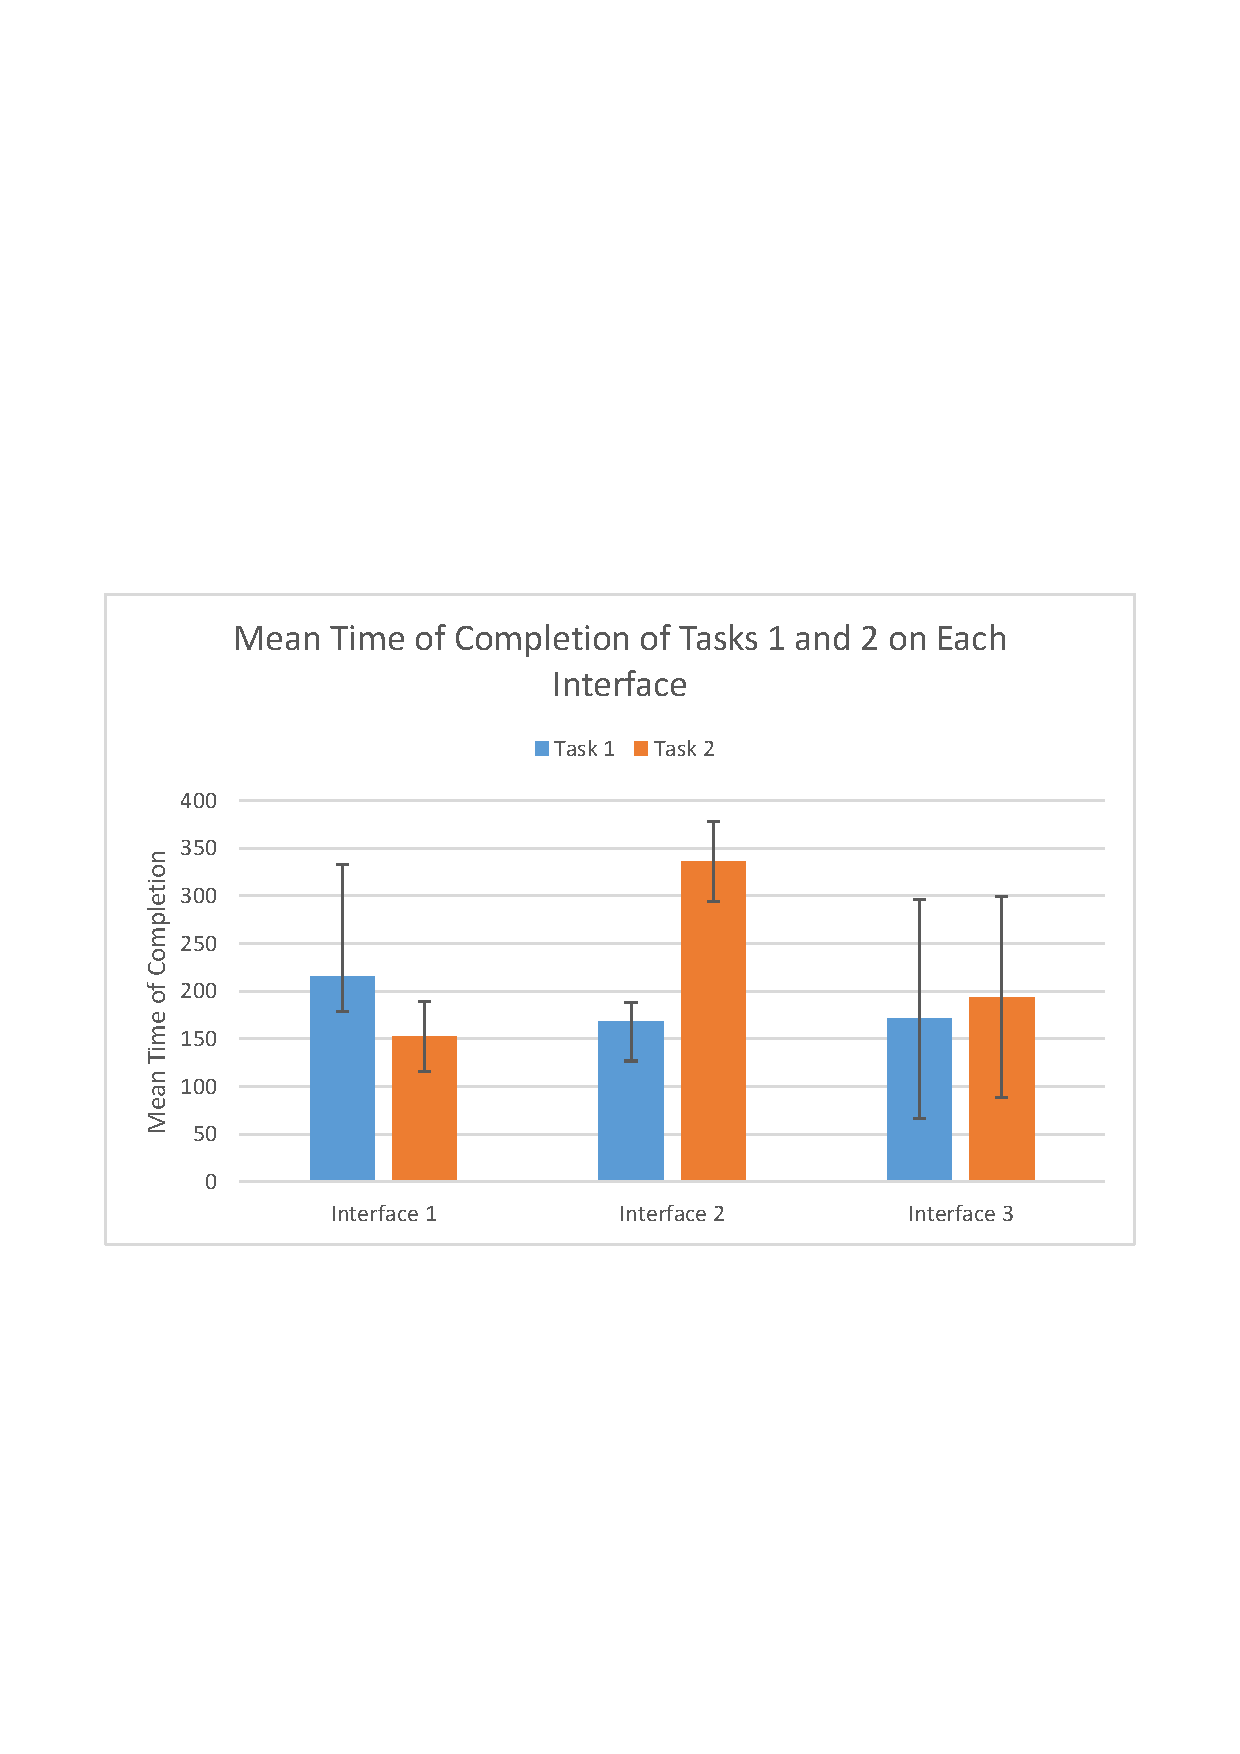
\includegraphics[width=\textwidth]{charts/table1.pdf}
		\caption{Mean Time Bar Graph}
		\label{ch:meantimebargraph}
	\end{subfigure}
	\begin{subfigure}{.5\textwidth}
		\centering
		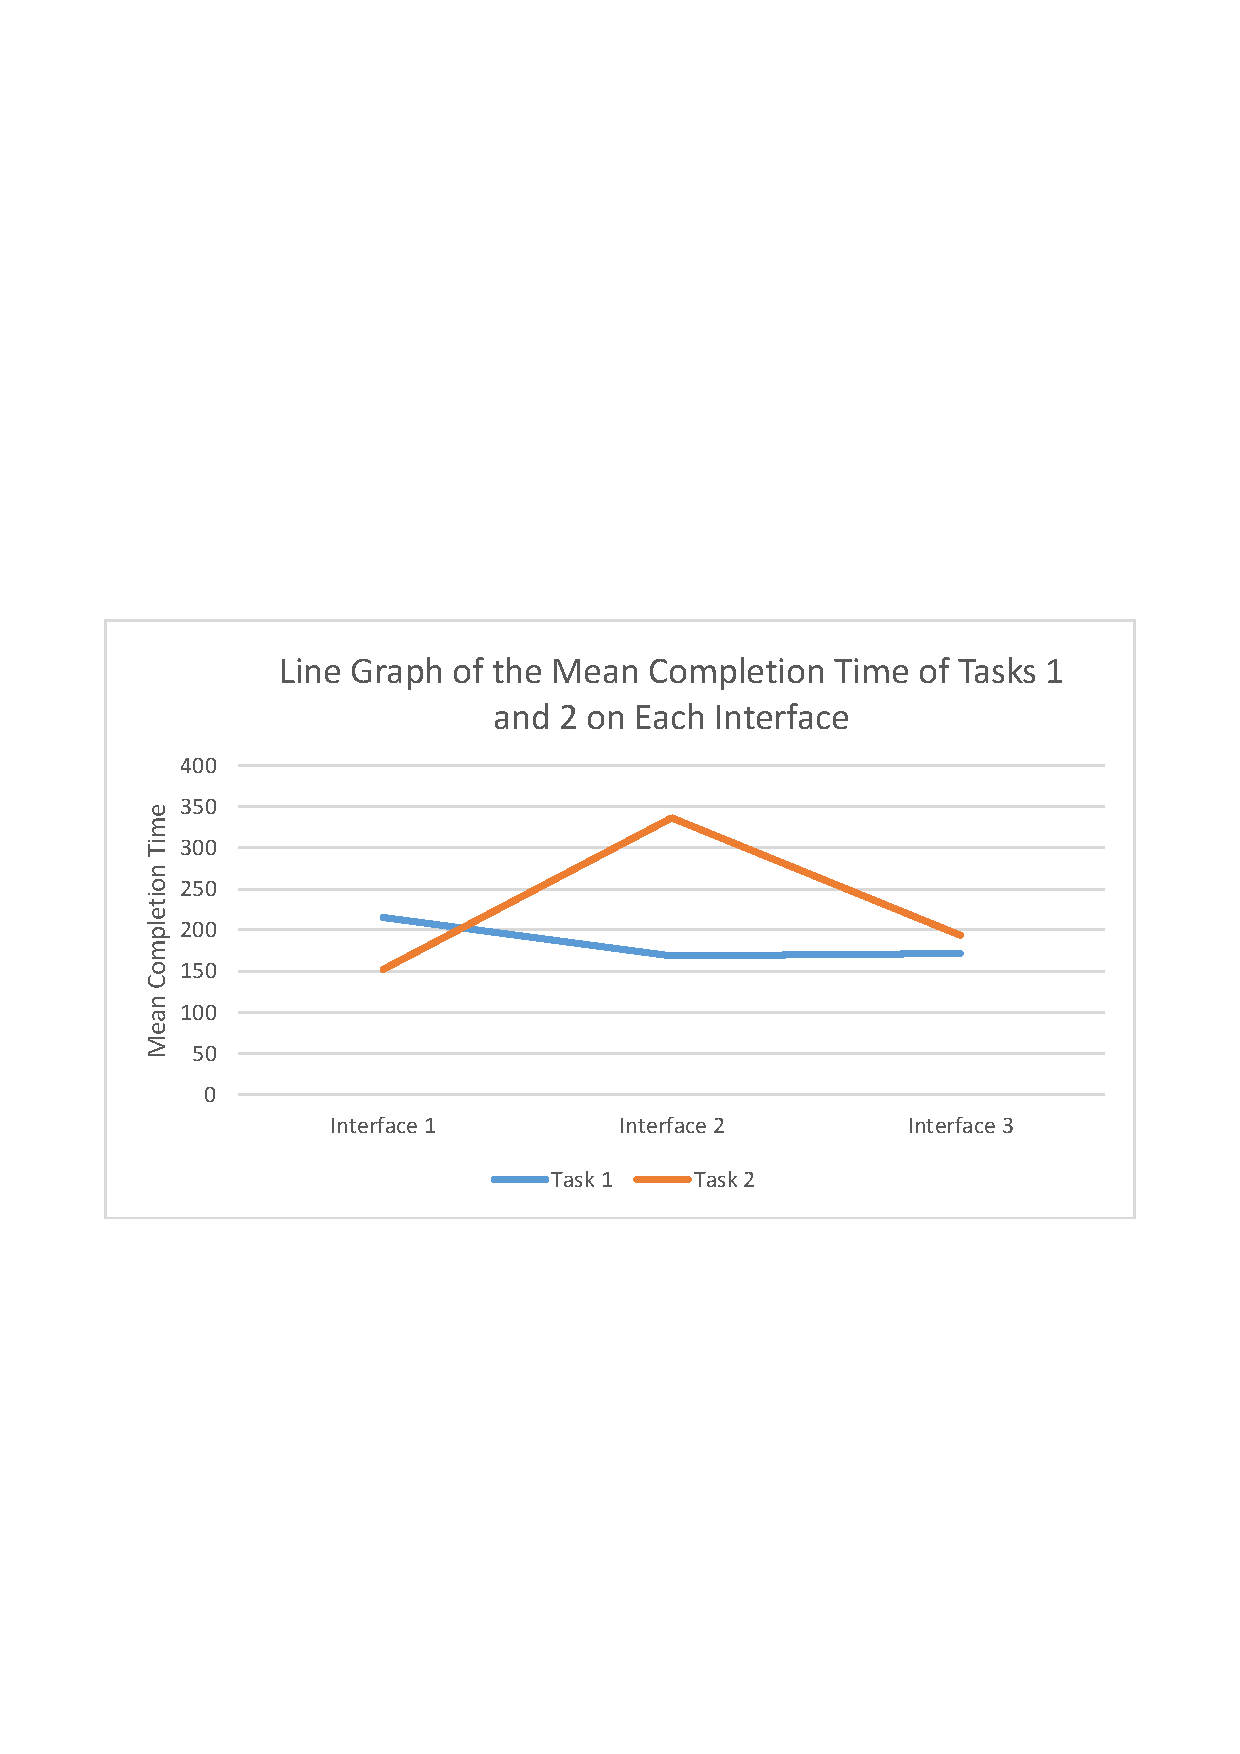
\includegraphics[width=\textwidth]{charts/table2.pdf}
		\caption{Mean Time Line Graph}
		\label{ch:meantimelinegraph}
	\end{subfigure}
	\caption{Results for Dependant Variable: Time}
	\label{fig:time}
\end{figure}

\paragraph{}
A 3x2 mixed factorial ANOVA was used to analyse the data. A significant interaction between Task and Interface was found (F(2,18)=5.058, p<0.05, η2=0.360). However, there were no significant main effect of Interface (F(2,18)=1.866, p=0.185, η2=0.172) an of Task (F(1,18)=1.903, p=0.185, η2=0.096). 
\paragraph{}
The second hypothesis suggested that there will be an interaction between Task and Interface on Total Number of Clicks. The mean number of clicks for completion of a task using a particular Interface were obtained and presented in Table \ref{tab:clickspertaskandinterface}. These were also illustrated along with errors bars for Standard Deviation in Figure \ref{ch:meantimebargraph}. As it is shown, Task 1 is on average completed with the least number of clicks on Interface 1 (M=21.50, SD=11.62), and largest number on Interface 2 (M=30.25, SD=2.754). The best mean value on Task 2 was also completed on Interface 1 (M=13.17, SD=0.753), and the highest mean value on Interface 2 (M=16, SD=1.826). The lowest total number of clicks required for completion of both tasks was obtained on Interface 1 (34.67). Furthermore, as it is illustrated in Figure \ref{ch:meanclicklinegraph}, when plotted on a line graph, there is no evidence of interaction. 


\begin{table}[H]
	\centering
	\begin{tabular}{|l|l|l|l|} \hline
		Task\textbackslash Interface Clicks(count)&	Interface 1	& Interface 2 &	Interface 3 \\ \hline
		Task 1 	& 21.50 (11.62)	& 30.25 (2.754)	& 27.00 (8.49)  \\ \hline
		Task 2	& 13.17 (0.753)	& 16.00 (1.826)	& 15.00 (2.828)  \\ \hline
		Total Clicks(count)	& 34.67	& 46.25 & 42.00 \\ \hline
	\end{tabular}
	\caption{Mean Number of Clicks for Task, performed on Interface}
	\label{tab:clickspertaskandinterface}
\end{table}

\begin{figure}[H]
	\begin{subfigure}{.5\textwidth}
		\centering
		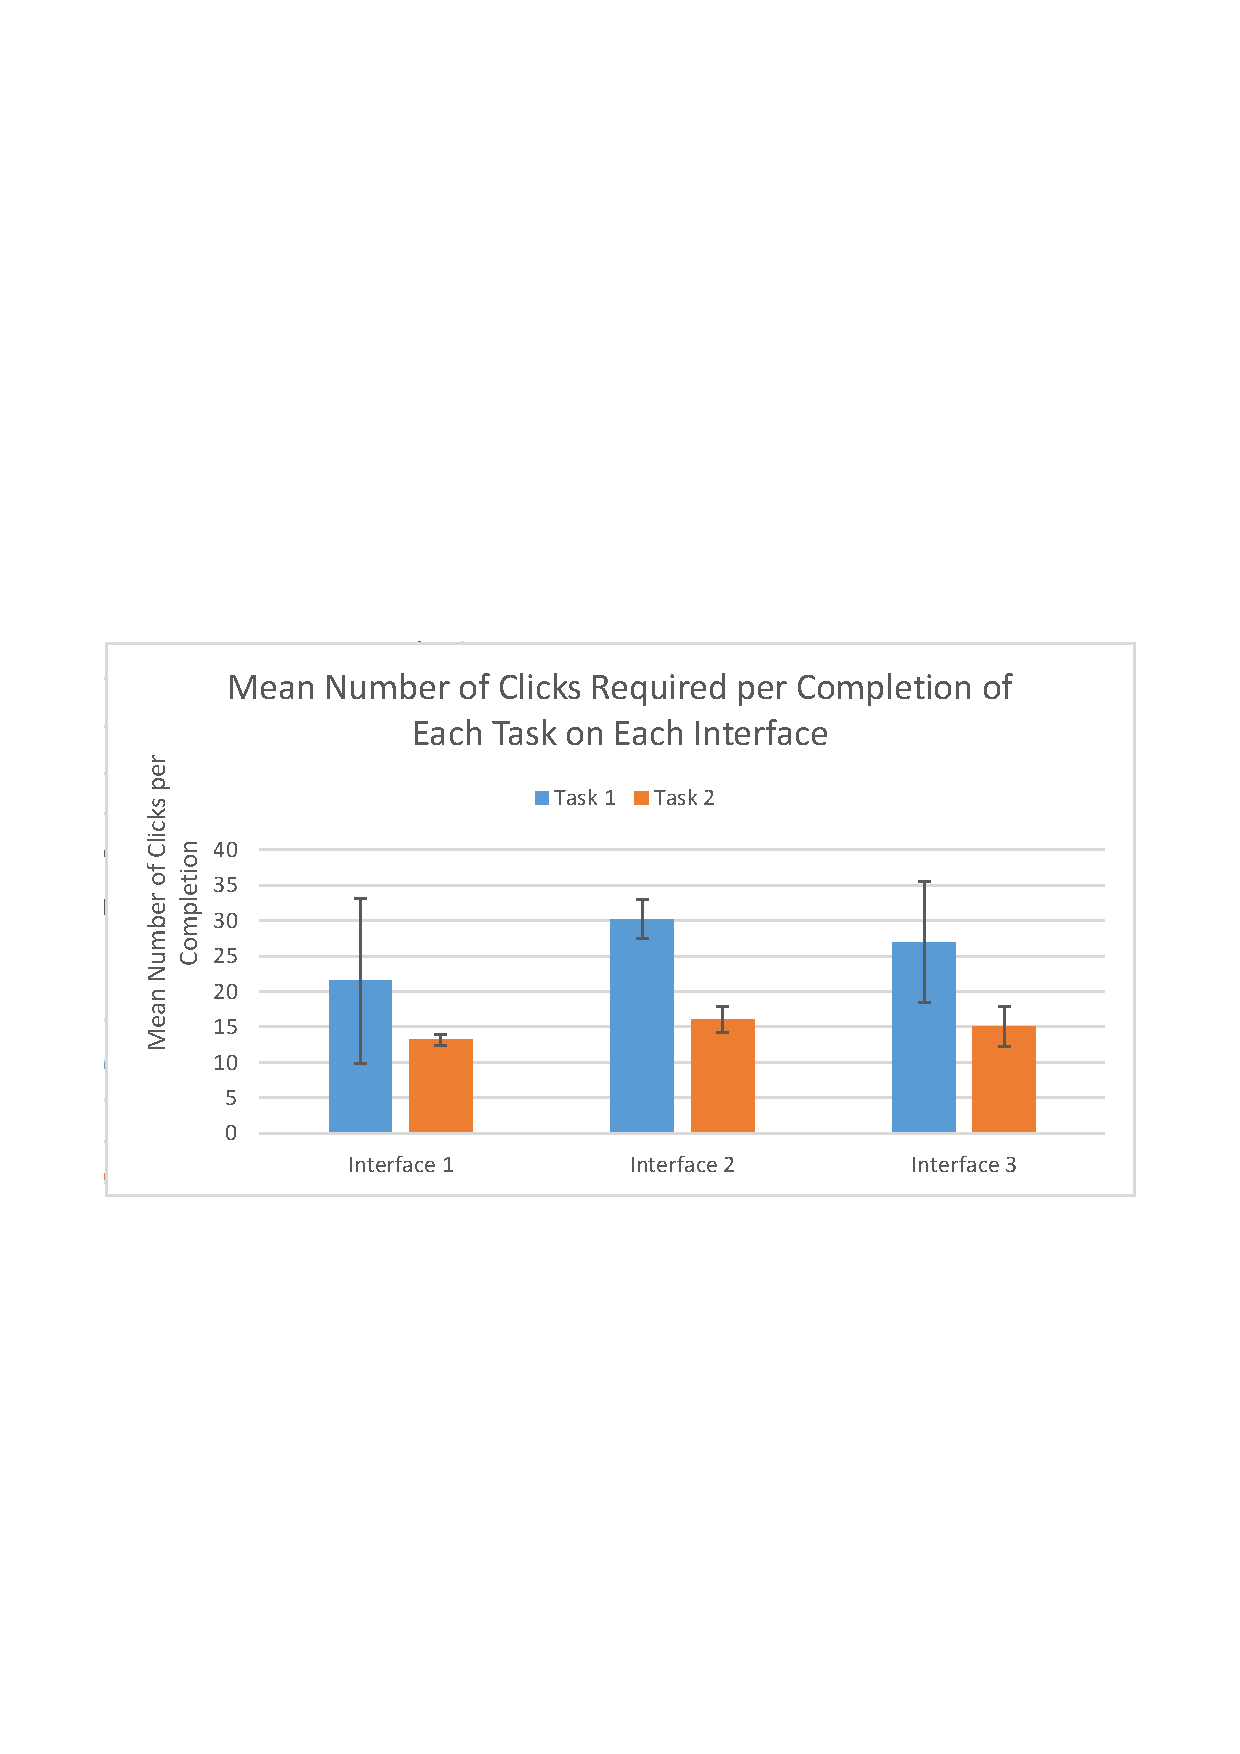
\includegraphics[width=\textwidth]{charts/table3.pdf}
		\caption{Mean Number of Clicks Bar Graph}
		\label{ch:meanclicksbargraph}
	\end{subfigure}
	\begin{subfigure}{.5\textwidth}
		\centering
		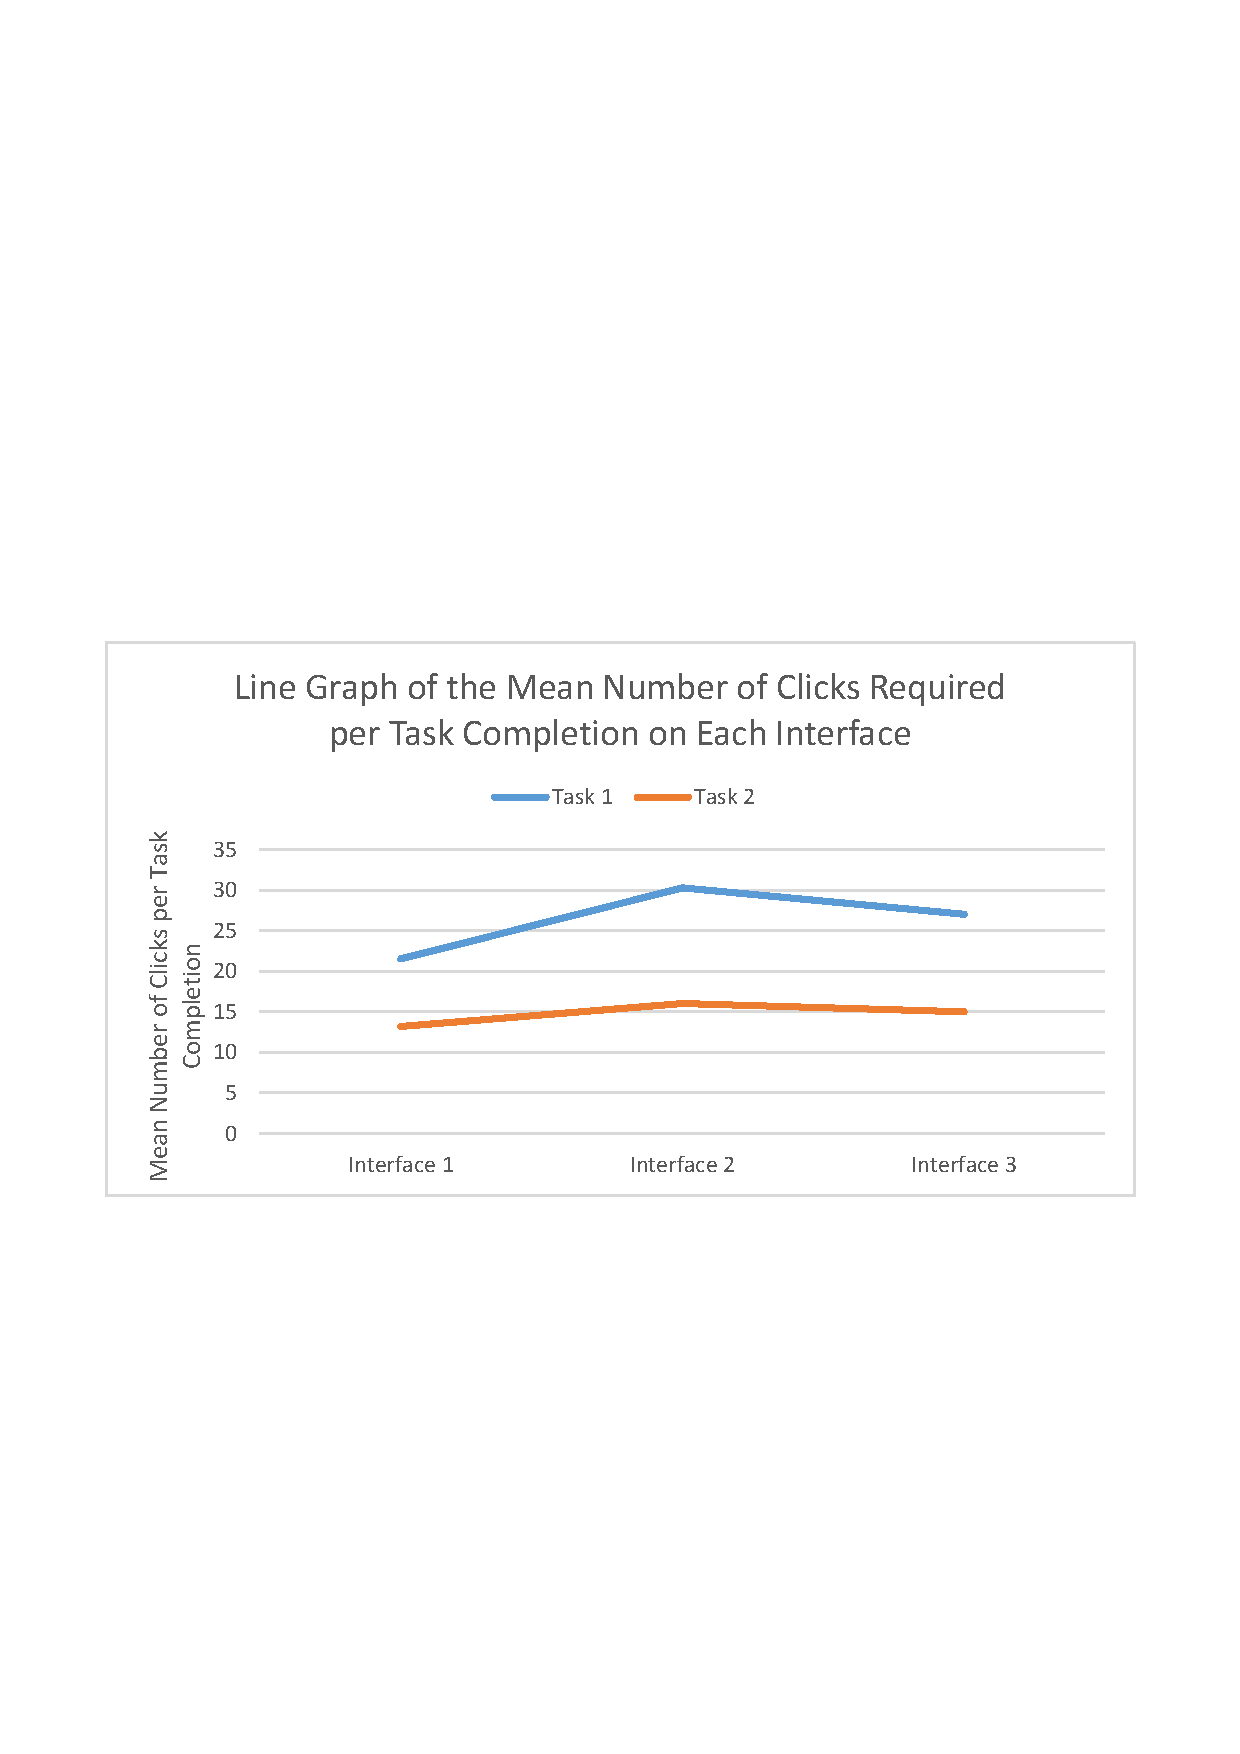
\includegraphics[width=\textwidth]{charts/table4.pdf}
		\caption{Mean Number of Clicks Line Graph}
		\label{ch:meanclicklinegraph}
	\end{subfigure}
	\caption{Results for Dependant Variable: Clicks}
	\label{fig:clicks}
\end{figure}
\paragraph{}
A second 3x2 mixed factorial ANOVA of Task (1*2) and Interface (1*2*3) was run to explore the number of clicks. No significant interaction between Task and Interface was found (F=(2,18), p=0.618, η2=0.052). Also there was no main effect of Interface on number of clicks per task completion (F=(2,18)=1.901, p=0.178, η2=0.174). However, a significant main effect of Task was found (F(1,18)=14.844, p<0.05, η2=0.52). 

\subsubsection{Results from Questionnaire}
\paragraph{}
All the participants had to complete the System Usability Scale questionnaire twice, once after each task and interface. For interface 1, representing the system with all the features, it was filled 12 times, for interface 2(the mobile version): 8 times and for interface 3(the version with the removed features): 4 times. Figure \ref{fig:susresultsmean} shows the scores after calculating the results. The biggest mean score is for interface 1(89.38), followed by interface 2(87.50) and interface 3(84.25). The fact that only 4 people filled in the questionnaire for interface 3 did not affect the overall score in this case as when further analysed, all of them had disagreed on the same statement: I found the various functions in this system were well integrated. In comparison, 3 of the them agreed and 1 strongly agreed on the same statement when asked for interface 1. On the other hand, the difference between interface 1 and 2 came from the fact that 4 participants disagreed on the first statement(I think that I would like to use this system frequently) after performing a task on the mobile version but agreed after using the full version. Finally, when asked, 8 participants said that they might not use the system as they did not use Twitter.

\begin{figure}[H]
	\centering
	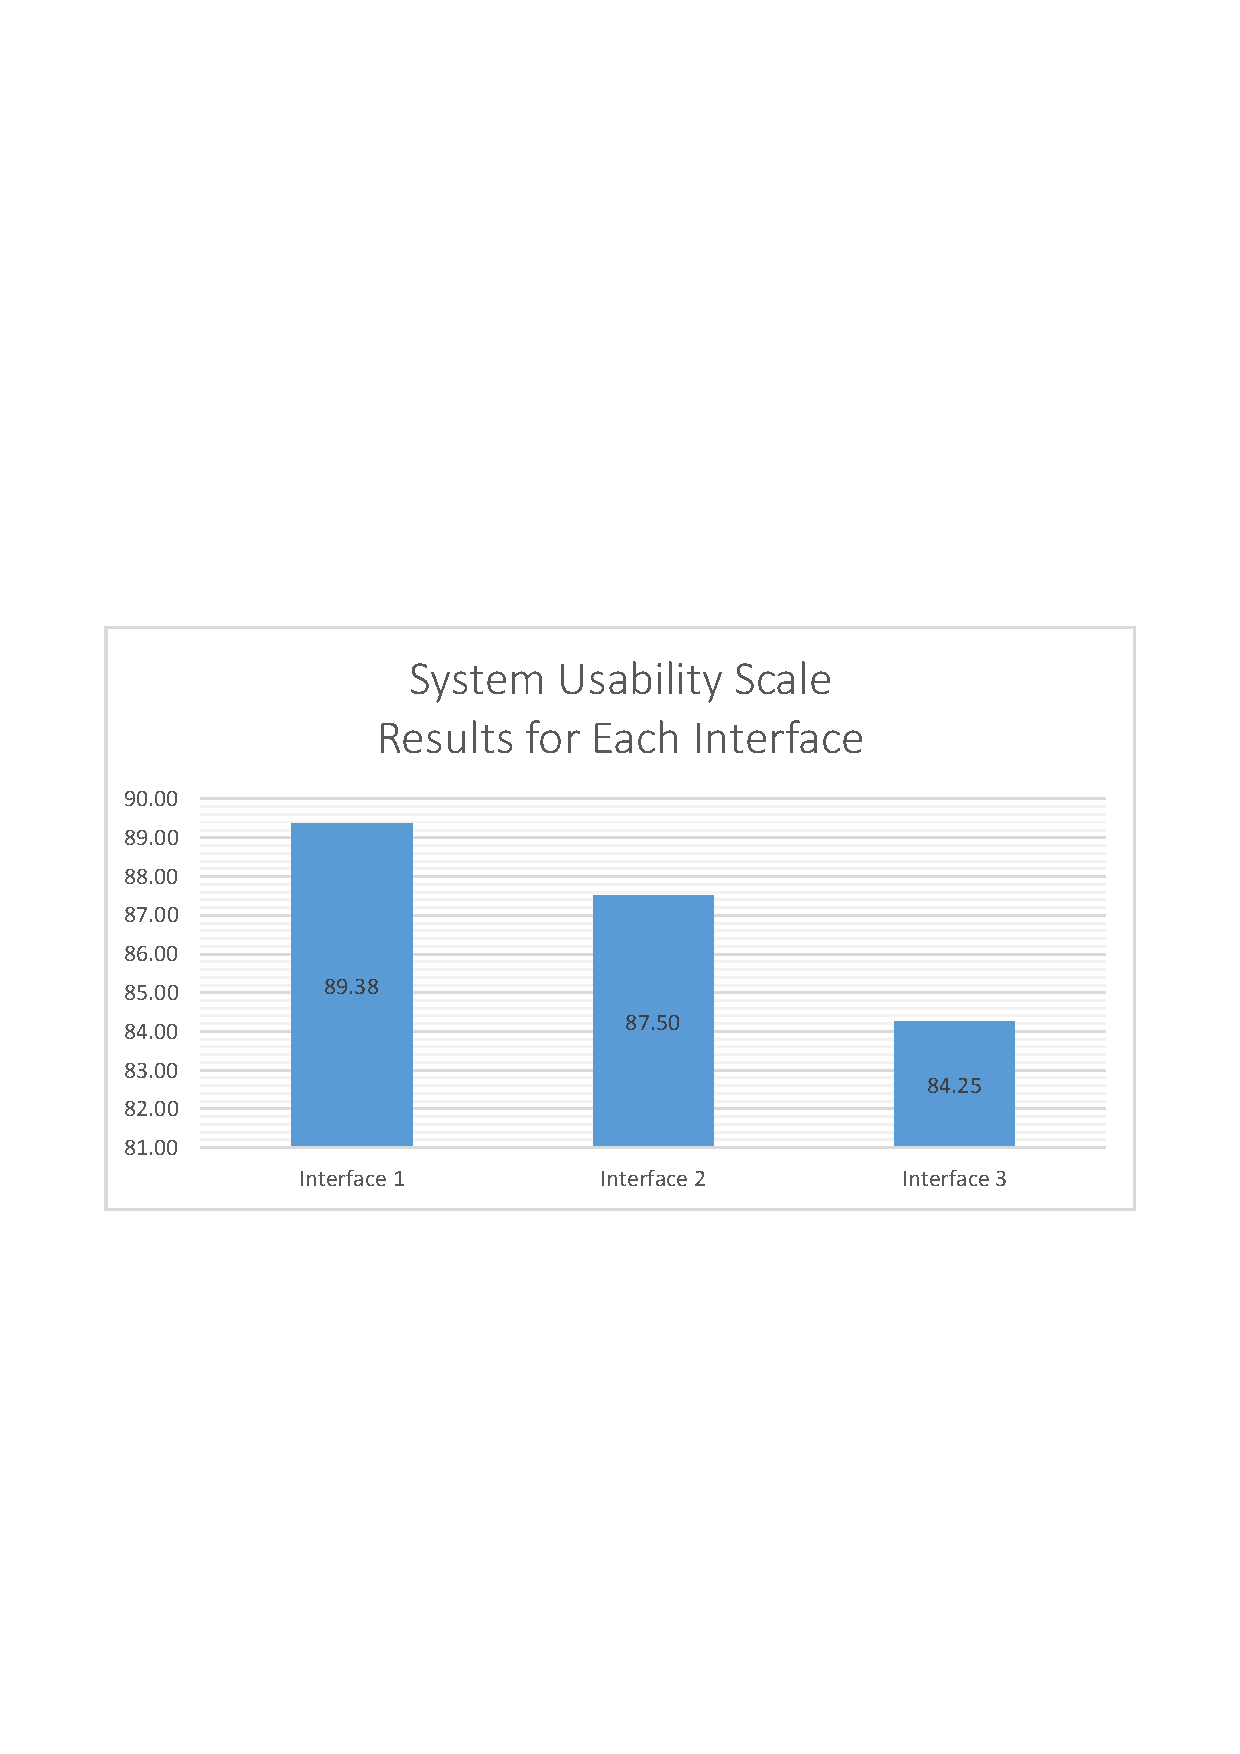
\includegraphics[width=.6\textwidth]{charts/SUSScaleMeanValues.pdf}
	\caption{SUS Scale Mean Values per Interface}
	\label{fig:susresultsmean}
\end{figure}

\subsubsection{Results from Think Aloud}
\paragraph{}
The Think Aloud was beneficial in two ways. First, it helped proving that the changes to the interface, performed after the initial phase of the evaluation,  were successful as none of the participants had any comments on the new separation of the components. Second, it helped identifying potential usability issues as well as comparing the different interfaces. 
\paragraph{}
Also, while performing tasks on interface 1, 4 participants said that the date input was not clear. The reason was that there were arrows and clearly written Day, Month and Year on the buttons but nothing was leading them to the conclusion that this was the place where they had to input a date. 3 participants were confused by the tweets and their text as they were not used to Twitter and the notion of multiple hash-tags. Additionally, when performing task 2, 5 participants made an error while inputting the venue in the search input box and 2 of them did not even notice the error message, returned from the system. Also, 6 participants were misled and thought that entering the venue in the location input box would lead them to the required place and did not take into account any chance for a difference in coordinates. 
\paragraph{}
Furthermore, while using interface 2 and performing task 2, 6 participants said that they had to scroll too much in order to reach the target and 2 of them suggested squeezing the timeline in case of too many tweets in a particular section and give the option to show more if required. 5 participants forgot which query corresponded to which timeline in the comparison screen due to the long scrolling and needed to go back to the top of the page. 3 people were confused from the Busy Venues events, which were displayed, and stated that there were no clues for showing the source of information. Furthermore, 4 participants felt it hard to find the place on the map as on mobile devices there is no hoover effect and only after pressing on the screen, they could have determine the venue that was selected. On the other hand, 6 participants liked the alignment of the timelines and the fact that they could be compared directly.
\paragraph{}
In addition, for interface 3, all of the participants directly noticed the lack of features and started looking for clues around the interface. They did not like the fact that there was no clear separation of the sections and that they had to follow the time-stamp on each event in order to determine the timeslot. Finally, all did not notice the lack of a graph but when asked, they pointed out that it was not needed for the particular task.

\subsubsection{Conclusion}
\paragraph{}
The results from the two ANOVA tests revealed that there is no significant effect of the interface, on its own, on the performance of the participants. However, due to the small sample size(12 people), the outcome of the experiment can not be generalised. Contrastingly, the analysis of the Questionnaire and Think Aloud evaluations revealed that the participants tend to prefer Interface 1, which represents the full system, due to its extra features. Finally, these results achieved the goal of the evaluation and showed that the implemented features were of value to the users.       

\section{Testing}
\paragraph{}
The functionality of the project was tested using white-box testing. This is a method that tests the internal components rather than the overall functionality. To design the tests, internal knowledge of the system was required. White-box testing can be used for both unit and integration tests.
\paragraph{}
Testing such application is a challenge. All the models talk to a service that is external to the system. However Laravel comes with built in Testing Component that allows for mocking objects and testing the views. Furthermore, for better coverage and reliability, both unit and integration tests were written to make sure that the application logic is consistent with the data, received from the services. Additionally, the interface was tested both manually and with unit tests. 

\subsection{Unit Tests}

\subsubsection{Testing Models}
\paragraph{}
To prepare each test, mocked sample response for the tested model was extracted form an original service response. Some of the values were modified so the tests can target specific behaviour of the tested Model. For example, the BusyVenue Model was tested against a response, containing three time series but only one was indicating that the venue was busy. This test asserted that the returned list with events from this model would be of length 1 and contained the exact time series. 

\subsubsection{Testing Interaction}
\paragraph{}
Additional to the manual interaction tests, unit tests were written during with the implementation to test both the navigation though the application and the validation of the input fields. This was time saving as there was no need for manually testing after a change had been done.  

\subsection{Integration Tests}

\subsubsection{Testing Models}
\paragraph{}
The models were tested in the same way as in the unit tests but this time using the actual response from the services. This insured that there were no changes to the format of the responses. Additionally, this was very important as the services were still under development and provided a quick way to check if an error came from the services or from the application logic.   

\subsubsection{Testing Json APIs}
\paragraph{}
Two RESTful APIs were implemented for this project but due to time constraints only one had been tested using integration tests. The Busy Venue API(reference to implementation) was tested against valid, wrong or missing GPS input. All the return messages were checked if they were appropriate depending on the given inputs.

\subsubsection{Testing Summary}
For the duration of this project, 26 tests with 84 assertions were written with overall test code coverage of 32.5\%.

\subsection{Manual Testing}
\paragraph{}
Both the initial and the final phases of the Evaluation process were used for performing manual testing. All the participants were given tasks to complete. As new users to the system, they were making mistakes. However, they did not manage to break the system but a few bugs were discovered. There were few cases when the timeline was not loading when there was an attempt to retrieve the venue's time series. Also, for a few participants, the two timelines in the comparison screen where not properly aligned but the problem was identified and fixed.

\section{Sonar}
\paragraph{}
SonarQube\footnote{http://www.sonarqube.org/} is an open platform that helps managing code quality. As such, it covers architecture \& design, comments, duplications, unit tests, complexity, potential bugs, coding rules, comments and sources. It is compatible with PHP as well. The required configuration was made so the project could be analysed and a report can be extracted. Figure \ref{fig:sonarreport} demonstrates how such a report looked like. It clearly shows the test coverage, percentage of duplications and how many lines of code had been written. Furthermore, if clicked on any of the rows, a more detailed report was displayed.  

\begin{figure}[H]
	\centering
	\includegraphics[width=.7\textwidth]{images/sonarreport}
	\label{fig:sonarreport}
	\caption{Sonar Report}
\end{figure}

\section{Summary}
\paragraph{}
To conclude, this chapter lists and explains the techniques, used for evaluating and testing the final product. Furthermore, it outlines possibilities for future improvements as well as identified problems. However, the next chapter expands on these findings and suggests possible solutions together with a summary of the whole project. 

\chapter{Conclusion}

\section{Future Work}
\paragraph{}
All the participants of the evaluation actively participated during the Think Aloud and helped to identify the following possible improvements, which they thought would improve the overall user experience.
\begin{itemize}
	\item \textbf{Scale}. The biggest issue, identified using the questionnaire, was that users might not use the system as they did not use Twitter. To try and increase the interest of this system, the best option is to add data from other social media portals like Facebook. Furthermore, the addition of data sources from different parts of the world might be beneficial as some of the events in Glasgow may be influenced by what is happening in a different country or continent.
	\item \textbf{Comparison variables} At this stage, the application allowed only for comparing tweets, which correspond to two hash-tags. For the future, users like researchers may benefit from a feature, that allows for comparing different variables or data streams between different dates.
	\item \textbf{Graphs} During the final evaluation, some of the participants, who were studying sociology or business, explained that they could benefit from different graph representations(Line graph or Scatter plot) of the results as they were used to tools like Excel or SPSS, which offer such functionality.  
	\item \textbf{Suggestions} Offering suggestions, based on the previous searches of the users, could lead to easier understanding of the capabilities of the system and what data it has to offer.
	\item \textbf{Interface improvements} The limitations of the user interface, identified in Section \ref{sub:finalphase}, should be addressed and most importantly the option to hide most of the events and allow for expanding a section by the user must be introduced so that the amount of scrolling can be drastically reduced.    
\end{itemize}

\section{Lessons Learnt}
\paragraph{}
The biggest lesson for the author was how to drive alone such a relatively big project from the initial planning up to the final evaluation. Furthermore, PHP had to be learnt in parallel with the progress on the project. Additionally, the authors knowledge about the model-view-controller as well as how the frameworks made use of this design pattern had increased significantly. 

\section{Summary}
\paragraph{}
This project aimed to build a tool for the fusion and visualisation of timely data. It went thought 23 iterations and 64 commits to the development branch in GitHub\footnote{https://github.com/skDn/Urban-Data-Timeline/tree/dev}. The final product was evaluated using 16 participants in total, who managed to prove that the application was usable by giving it a very high usability score of 89.38(Figure: \ref{fig:susresultsmean}) out of 100. Furthermore, the received verbal feedback confirmed that the implemented features were valuable to the users. 

\section{Acknowledgements}
I would like to thank Dr. Iadh Ounis and Dr. Craig Macdonald for supervising this project and providing their very valuable feedback when required. Furthermore, many thanks to the Urban Big Data Centre for making this project possible by providing part of the data, collected for their Integrated Multimedia City Data project, and to Dr. Sean Moran, who was developing and supporting the services that were giving me access to the data. Finally, I would like to thank all of the participants, who took part in the evaluation, as their performance and feedback managed to prove that the final product was successful.  

%%%%%%%%%%%%%%%%
%              %
%  APPENDICES  %
%              %
%%%%%%%%%%%%%%%%
\begin{appendices}
	\chapter{Progress Reports}
	\includepdf[pages=-]{meetings/progress1.pdf}
	\includepdf[pages=-]{meetings/progress2.pdf}
	\includepdf[pages=-]{meetings/progress3.pdf}
	\includepdf[pages=-]{meetings/progress4.pdf}
	\includepdf[pages=-]{meetings/progress5.pdf}
	\includepdf[pages=-]{meetings/progress6.pdf}
	\includepdf[pages=-]{meetings/progress7.pdf}
	\includepdf[pages=-]{meetings/progress8.pdf}
	\includepdf[pages=-]{meetings/progress9.pdf}
	\includepdf[pages=-]{meetings/progress10.pdf}
	\includepdf[pages=-]{meetings/progress11.pdf}
	\includepdf[pages=-]{meetings/progress12.pdf}
	\includepdf[pages=-]{meetings/progress13.pdf}
	\includepdf[pages=-]{meetings/progress14.pdf}
	\includepdf[pages=-]{meetings/progress15.pdf}
	\includepdf[pages=-]{meetings/progress16.pdf}
	\includepdf[pages=-]{meetings/progress17.pdf}
	\includepdf[pages=-]{meetings/progress18.pdf}
	\includepdf[pages=-]{meetings/progress19.pdf}
	\includepdf[pages=-]{meetings/progress20.pdf}
	\includepdf[pages=-]{meetings/progress21.pdf}
	\includepdf[pages=-]{meetings/progress22.pdf}
	\chapter{Evaluation Raw results}
	\clearpage
	\begin{minipage}{\textwidth}
		\section{Time}
		\includepdf[pages=1]{apendix/evaluationresults.pdf}
	\end{minipage}
	\clearpage
	\begin{minipage}{\textwidth}
		\section{Clicks}
		\includepdf[pages=2]{apendix/evaluationresults.pdf}
	\end{minipage}
	\chapter{Evaluation Documents}
	\clearpage
	\begin{minipage}{\textwidth}
		\section{Consent}
		\includepdf[pages=-]{apendix/consent.pdf}
	\end{minipage}
	\clearpage
	\begin{minipage}{\textwidth}
		\section{Introduction and Debrief scripts}
		\includepdf[pages=1]{apendix/evaluationdocs.pdf}
	\end{minipage}
	\clearpage
	\begin{minipage}{\textwidth}
		\section{Task sheet}
		\includepdf[pages=2]{apendix/evaluationdocs.pdf}
	\end{minipage}
	\clearpage
	\begin{minipage}{\textwidth}
		\section{Questionnaire}
		\includepdf[pages=3]{apendix/evaluationdocs.pdf}
	\end{minipage}
	\clearpage
	\begin{minipage}{\textwidth}
		\section{Setup guide}
		\includepdf[pages=-]{apendix/setup.pdf}
	\end{minipage}
	
\end{appendices}

%%%%%%%%%%%%%%%%%%%%
%   BIBLIOGRAPHY   %
%%%%%%%%%%%%%%%%%%%%

\bibliographystyle{plain}
\bibliography{bib}

\end{document}
